\chapter{Simulation Environment}

The Environment page defines the initial conditions and simulation time for the CFAST input file.

\begin{figure}[ht]
\centering
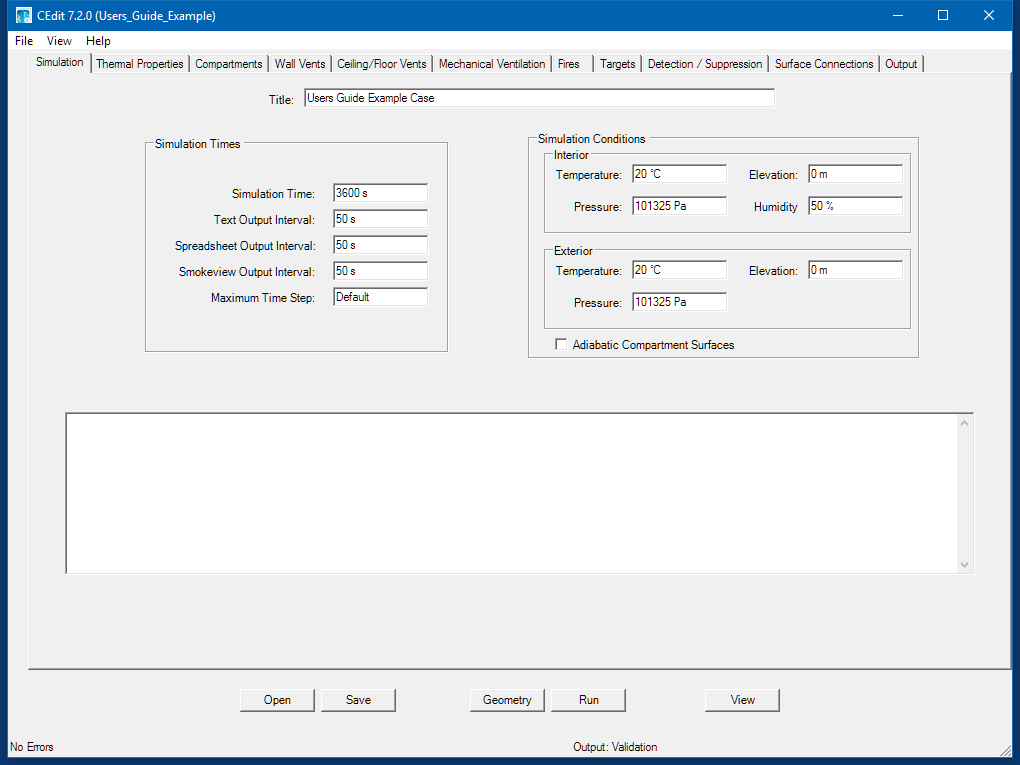
\includegraphics[width=6.5in]{FIGURES/Environment_Tab}
\caption[The CFAST Simulation Environment Tab]{The CFAST Simulation Environment Tab.}
\end{figure}

\section{Version and Title}
\label{info:HEAD}

\begin{description}
\item[Version] The version of CFAST being used by the user. Version number can be found in the upper left corner in the CEdit user interface as shown in Fig. \ref{Figure 1.1}.

\item[Title] The first thing to do when setting up an input file is to give the simulation a title. The title is optional and may consist of letters, numbers, and/or symbols and may be up to 50 characters. All output files will be tagged with this character string.
\end{description}




\section{Simulation Times}
\label{info:TIME}

\begin{description}
\item[Simulation Time] (default units: s, default value, 900 s): The length of time over which the simulation takes place. The maximum value for this input is 86400 s (1 day).

\item[Text Output Interval] (default units: s, default value, 60 s): The time interval between each printing of the output data.  If equal to zero, no output values will appear.

\item[Spreadsheet Output Interval] (default units: s, default value, 15 s): CFAST can output the results of the simulation in a set of comma-delimited spreadsheet files. This parameter defines the time interval between these outputs. A value greater than zero must be used if the spreadsheet files are desired.

\item[Smokeview Output Interval] (default units: s, default value: 15 s): CFAST can output a subset of the results in a format compatible with the visualization program Smokeview. This input defines the time interval between outputs of the model results in a Smokeview-compatible format.  A value greater than zero must be used if the Smokeview output is desired.

\item[Maximum Time Step] (default units: s, default value: 2 s): CFAST will automatically adjust the time interval for the solution of the differential equation set up or down so that the simulation is as efficient as possible within the pre-defined error tolerances. This parameter places a maximum value for the equation solver and can normally be left at the default value. In cases (which are hopefully rare) where the model fails to converge on a solution, this value can be reduced which often will allow the simulation to successfully complete.
\end{description}




\section{Simulation Conditions}
\label{info:INIT}

Ambient conditions define the environment at which the scenario begins. Initial pressures in a structure are calculated simply as a lapse rate (related to the height above sea level) based on the NOAA/NASA tables \cite{GPO:Atmosphere}. It is convenient to choose the base of a structure to be at zero height and then reference the height of the structure with respect to that height.  The temperature and pressure must then be measured at that position.  Another possible choice would be the pressure and temperature at sea level, with the structure elevations then given with respect to mean sea level.  This is also acceptable, but somewhat more tedious in specifying the construction of a structure.  Either of these choices works though, so long as they are consistent. Usually, the station elevation is set to zero and the pressure to ambient. The effect of changing these values is minor. Note that the equations implemented in the model are not designed to handle negative elevations and altitudes.

\begin{description}
\item[Temperature] (default units: \degc, default value: 20 \degc): Initial ambient temperature inside the structure at the station elevation.

\item[Humidity] (default units \% RH, default value: 50 \%): The initial relative humidity in the system, only specified for the interior.  This is converted to kilograms of water per cubic meter as an initial condition for both the interior and exterior of the structure.

\item[Temperature] (default units: \degc, default value: 20 \degc): Initial ambient temperature outside the structure at the station elevation.

\item[Pressure] (default units: Pa, default value: 101325 Pa): Initial values for ambient atmospheric pressure inside and outside the structure at the station elevation. The default value is standard atmospheric pressure at sea level.
\end{description}


\section{Miscellaneous}
\label{info:MISC}

Keywords associated to global parameters are organized in the miscellaneous namelist group.

\begin{description}
\item[Adiabatic Compartment Surfaces] When this box is checked, all of the compartment surfaces are assumed to be perfect insulators and the materials section of the compartments tab becomes grayed out. This feature is useful when designing an experiment in which it is safe to assume that there is no heat transfer to the walls of the compartments.

\item[Lower Oxygen Limit] (default units: \%, default value: 15~\%):  In the CFAST model, a limit is incorporated by limiting the burning rate as the oxygen level decreases until a ``lower oxygen limit'' (LOL) is reached. The lower oxygen limit is incorporated through a smooth decrease in the burning rate near the limit. Normally, this value would not be changed by the user.
\end{description}





\chapter{Thermal Properties}

The thermophysical properites of materials used for compartment surfaces or targets are set in the Thermal Properties tab.

\begin{figure}[ht]
\centering
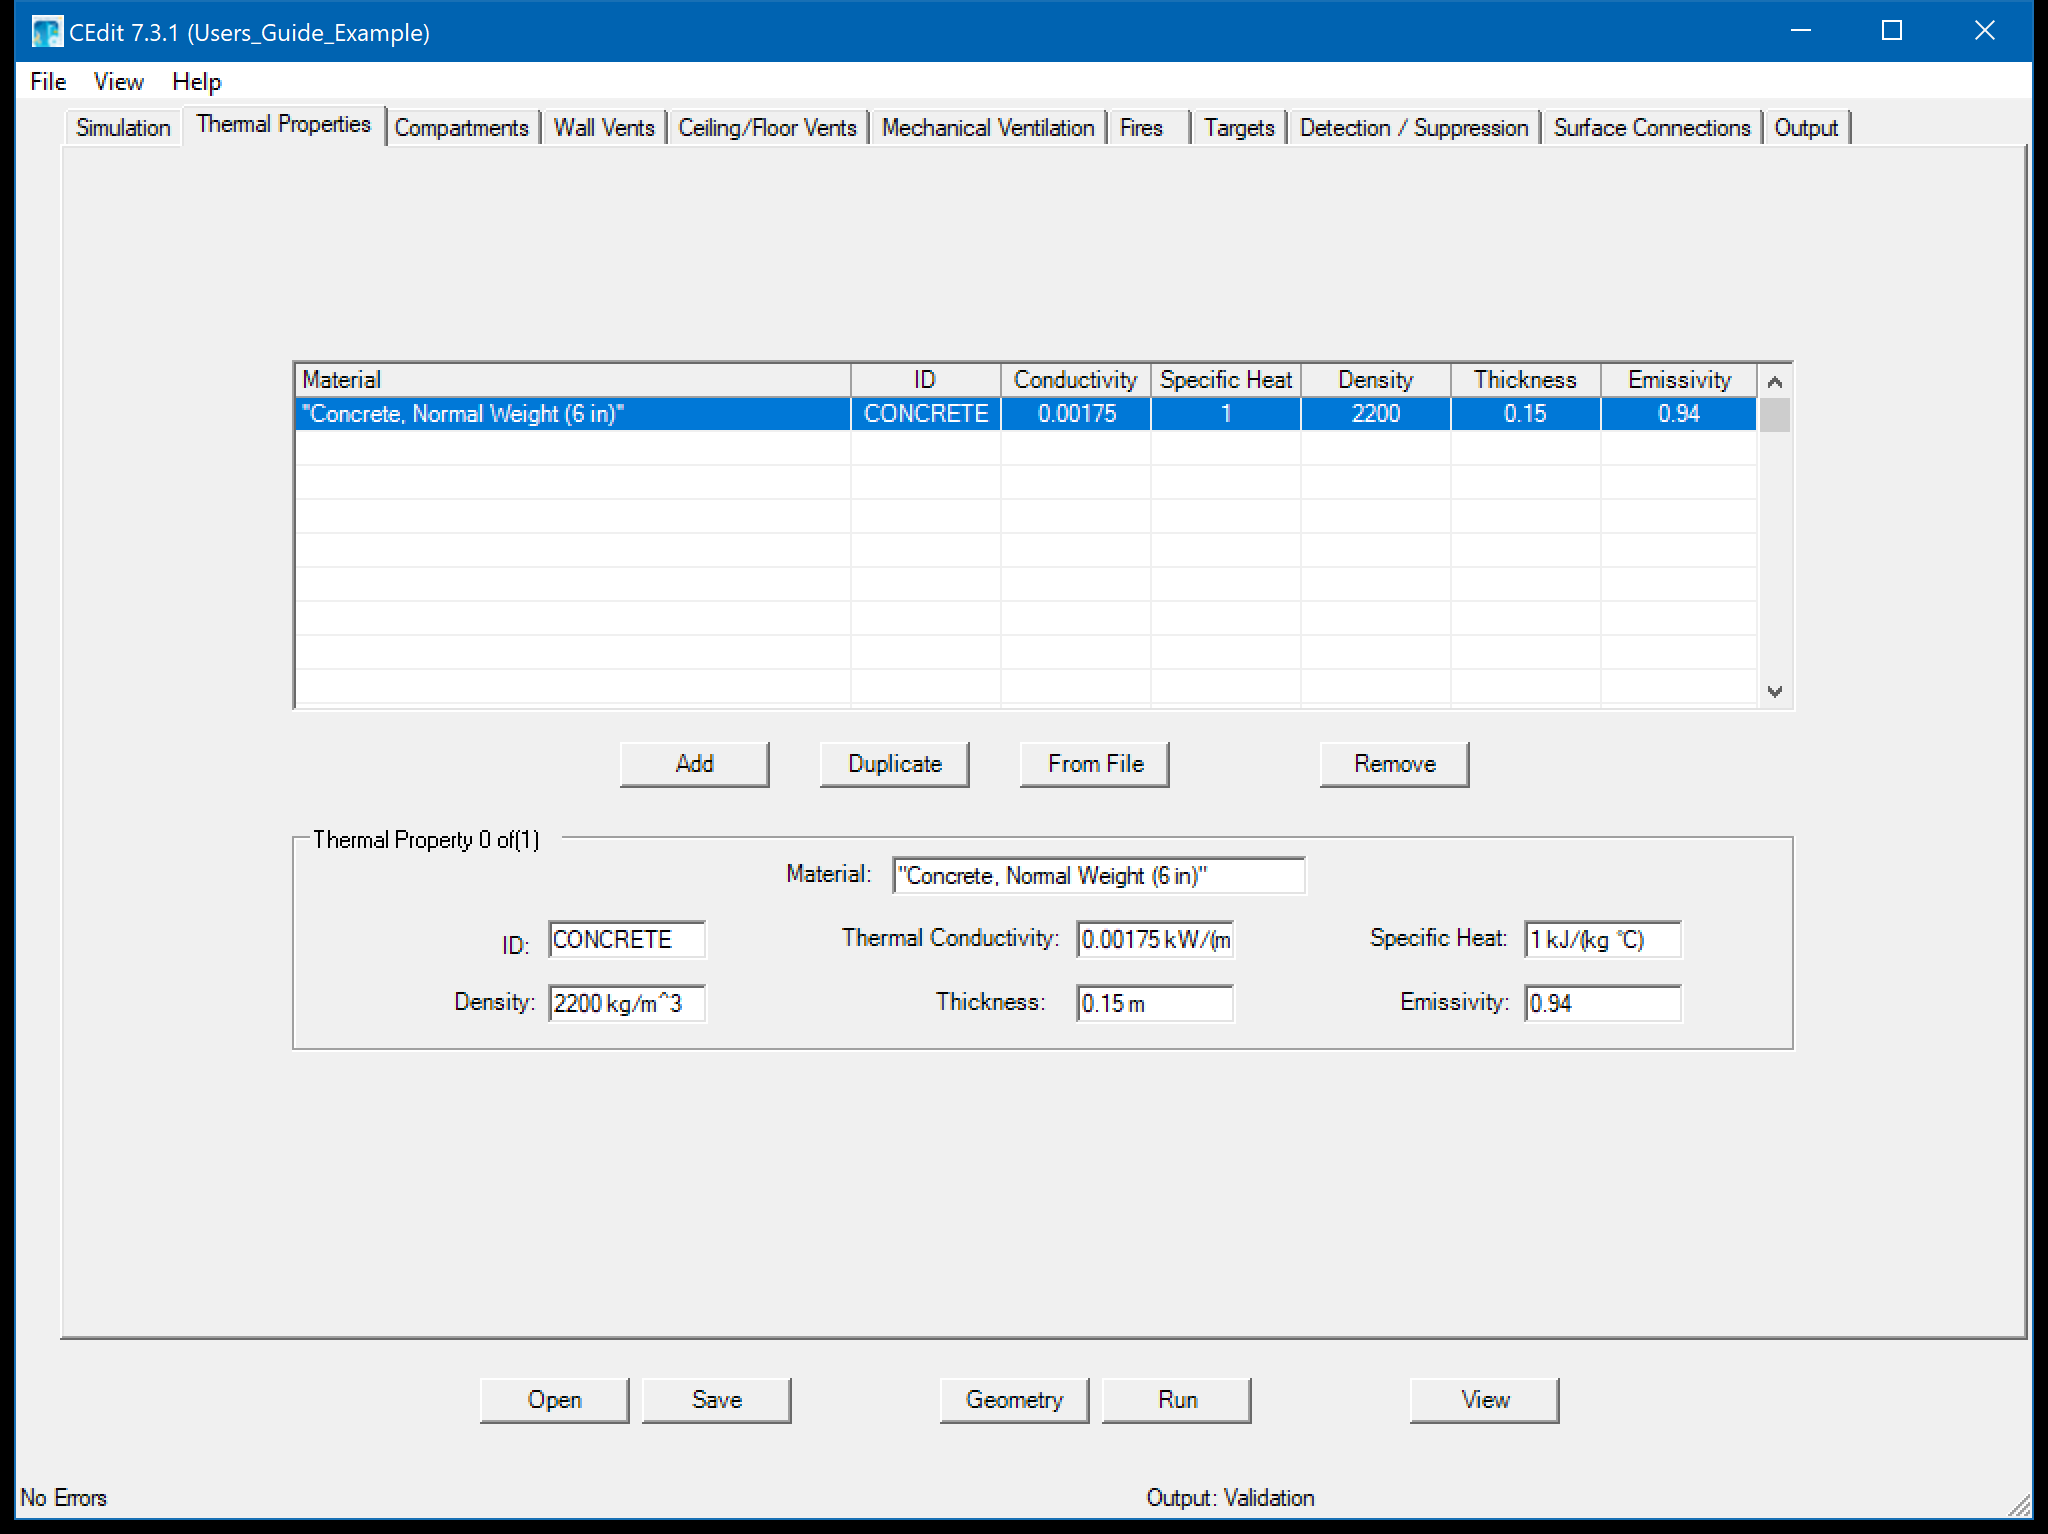
\includegraphics[width=6.5in]{FIGURES/Thermal_Properties_Tab}
\caption[The CFAST Thermal Properties Tab]{The CFAST Thermal Properties Tab.}
\end{figure}

\section{Adding Thermal Properties}
\label{info:MATL}

CFAST and CEdit do not include predefined thermal properties for compartment materials. Thus, the user needs to define materials for use within a specific simulation. These may be from other simulations or input directly from reference sources or test results. Clicking the `Add' button and assigning values to the following list of properties will create a set of thermal properties associated with a material used in a compartment or a target. The thermophysical properties are specified at one condition of temperature, humidity, etc.  Only a single layer per boundary is allowed (some previous versions allowed up to three).

\begin{description}
\item[Material] A descriptive name for the material.

%% Do we want to change the requirements on the ID. We don't have those requirements in the Name List
\item[ID] A one-word (no more than 8 characters) \textbf{unique} identifier for the material.  This identifier should not contain any spaces and is used in other CFAST inputs to identify the particular material referenced.

\item[Conductivity] (default units: kW/(m$\cdot$\degc)  or  kW/(m$\cdot$K)): Thermal conductivity for the material.

\item[Specific Heat] (default units: kJ/(kg$\cdot$\degc) or kJ/(kg$\cdot$K)): Specific heat for the material.

\item[Density] (default units: kg/m$^3$): Density for the material.

\item[Thickness] (default units: m): Thickness of the material.  Note that if two materials with identical thermal properties but with different thicknesses are desired, two separate materials must be defined.

\item[Emissivity] (default units: none, default value: 0.9): Emissivity of the material surface.  This is the fraction of radiation that is absorbed by the material.
\end{description}




\section{Adding Thermal Properties From Another File}

The `From File' button allows you to insert thermal properties from existing CFAST input files to the current simulation.

\begin{figure}[h!]
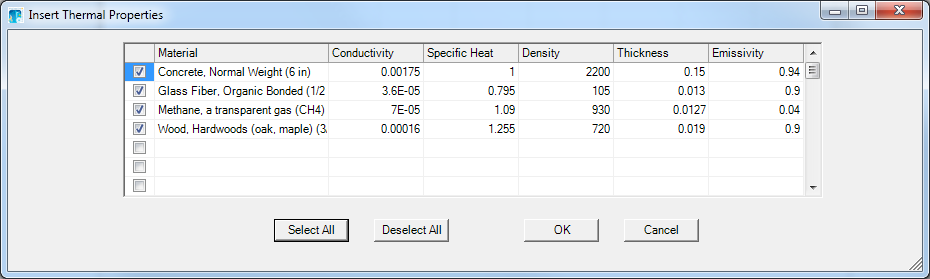
\includegraphics[width=6.5in]{FIGURES/Insert_Thermal_Properties}
\caption[Inserting Thermal Properties in CFAST]{Inserting Thermal Properties in CFAST.}
\end{figure}





\chapter{Compartments}
\begin{figure}[h!]
\begin{center}
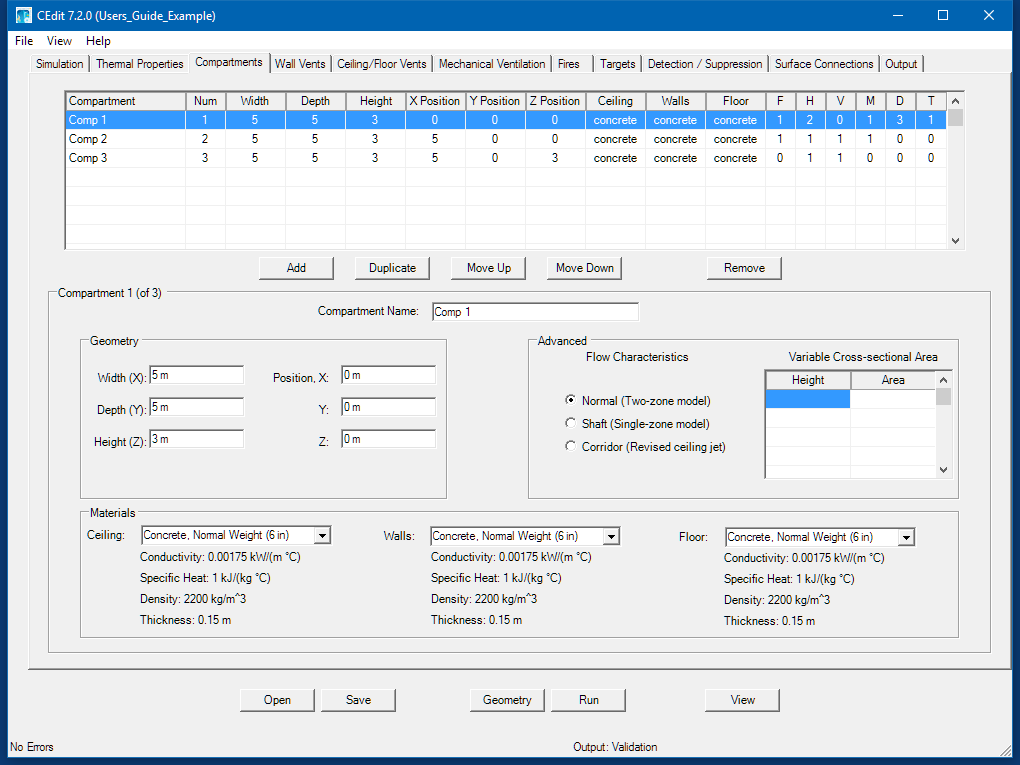
\includegraphics[width=6.5in]{FIGURES/Compartment_Geometry_Tab}
\caption[The CFAST Compartments Tab]{The CFAST Compartments Tab.}
\end{center}
\end{figure}

The Compartments page defines the size, position, materials of construction, and flow characteristics for the compartments in the simulation. Initially, only the simulation environment page and the 'Add' button on the compartment geometry and thermal properties pages are enabled; all other pages are not available to the user for detailed inputs until a compartment has been added to the simulation.

In order to model a fire scenario, the size and position of each compartment relavent to the scenario must be specified. For a compartment, the width, depth, compartment height and height of the floor of the compartment provide this specification. The maximum number of compartments for version 7 is 100. The usual assumption is that compartments are rectangular parallelepipeds. However, the CFAST model can accommodate odd shapes as equivalent floor area parallelepipeds or with a cross-sectional area that varies with height.

\begin{figure}[h!]
\begin{tabular*}{\textwidth}{c@{\extracolsep{\fill}}c}
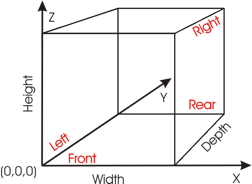
\includegraphics[width=2.5in]{FIGURES/CFAST_Coordinates} &
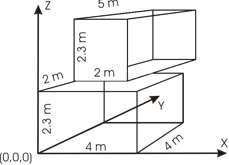
\includegraphics[width=2.6in]{FIGURES/CFAST_Absolute_Positioning} \\
Compartment Size & Compartment Position
\end{tabular*}
\caption[Compartment Orientation and Positioning in CFAST]{Compartment Orientation and Positioning in CFAST.}
\label{fig:compartment_positioning}
\end{figure}

In CEdit the default size of a room has width of 3.6 m, depth of 2.4 m, and height of 2.4 m. There are defaults for absolute positioning (0,0,0). All surfaces, i.e., the ceiling, walls and floor, are turned off by default. The fully mixed (single zone) and corridor models are turned off by default.

\label{Compartment_Geometry}Compartments in CFAST are most typically defined by a width, depth, and height.  If desired, compartments can be prescribed by the cross-sectional area of the compartment as a function of height from floor to ceiling for other shapes. The absolute position of the compartment with respect to a single structure reference point can be defined to ease visualization or to allow exact placement of vents and surfaces relative to other compartments in a detailed calculation. This specification is important for positioning the compartments for visualization in Smokeview.

\begin{description}
\item[ ID:] Compartments are identified by a unique alphanumeric name.  This may be as simple as a single character or number, or a description of the compartment.
\end{description}




\section{Geometry}
\label{info:COMP}
\begin{description}
\item[Width] (default units m, default value 3.6 m) specifies the width of the compartment as measured on the X axis from the origin (0,0,0) of the compartment.

\item[Depth]  (default units m, default value 2.4 m) specifies the depth of the compartment as measured on the Y axis from the origin (0,0,0) of the compartment.

\item[Height] (default units m, default value 2.4 m)  specifies the height of the compartment as measured on the Z axis from the origin (0,0,0) of the compartment.

\item[Position X] (default units m, default value 0.0 m)  specifies the absolute x coordinate of the lower, left, front corner of the room. All absolute positions for all compartments must be greater than or equal to zero, i.e., negative numbers are not allowed for these inputs. Important in positioning the compartments for visualization in Smokeview.

\item[Position Y] (default units m, default value 0.0 m)  specifies the absolute y coordinate of the lower, left, front corner of the room. All absolute positions for all compartments must be greater than or equal to zero, i.e., negative numbers are not allowed for these inputs. Important in positioning the compartments for visualiz
ation in Smokeview.

\item[Position Z] (default units m, default value 0.0 m)  specifies the height of the floor of each compartment with respect to station elevation specified by the internal ambient conditions reference height parameter.  The reference point must be the same for all elevations in the input data.  For example, the two rooms in the sample to the right in Fig.~\ref{fig:compartment_positioning} would be located at (0,0,0) and (0,2,2.3). All absolute positions for all compartments must be greater than or equal to zero, i.e., negative numbers are not allowed for these inputs.
\end{description}




\section{Materials}
\label{info:COMP2}
To calculate heat loss through the ceiling, walls, and floor of a compartment, the properties of the bounding surfaces must be known. This includes the thermophysical properties of the surfaces and the arrangement of adjacent compartments if inter-compartment heat transfer is to be calculated.
The bounding surfaces are the ceilings, walls and floors that define a compartment. These are referred to as thermophysical boundaries, since each participates in conduction, convection, and radiation as well as defining the compartments, unless these phenomena are explicitly turned off.

The thermophysical properties of the materials to be used to define the surfaces are defined in the Thermal Propertied tab described in section \ref{info:MATL}. The materials are then assigned to the ceiling, wall, and floor surfaces by use of the material ID

\begin{description}
\item[Ceiling Material] (default value: Off): up to three materials from the thermal properties from the Materials tab can be used to define the layer(s) of the ceiling surface of the compartment. The innermost layer is specified first.

\item[Ceiling Thickness] (default units: m, default value: thickness of material specified on the Materials tab): thickness of each of the layers of the ceiling surface.

\item[Wall Material] (default value: Off): up to three materials from the thermal properties from the Materials tab can be used to define the layer(s) of the wall surface of the compartment.  The innermost layer is specified first.

\item[Wall Thickness] (default units: m, default value: thickness of material specified on the Materials tab): thickness of each of the layers of the ceiling surface.

\item[Floor Material] (default value: Off): up to three materials from the thermal properties from the Materials tab can be used to define the layer(s) of the floor surface of the compartment.  The innermost layer is specified first.

\item[Floor Thickness] (default units: m, default value: thickness of material specified on the Materials tab): thickness of each of the layers of the floor surface.
\end{description}

\graybox{
If the thermophysical properties of the enclosing surfaces are not included, CFAST will treat them as adiabatic (no heat transfer). \\

If a name is used which is not in the input file, the model should stop with an error message. \\

The back surfaces of compartments are assumed to be exposed to ambient conditions unless specifically specified (see the section on Surface Connections to specify heat transfer connections between compartments).
}




\section{Modeling a Compartment as a Tall Shaft or Long Corridor}
\label{info:COMP3}
For tall compartments or those removed from the room of fire origin, the compartment may be modeled as a single, well-mixed zone rather than the default two-zone assumption. A single zone approximation is appropriate for smoke flow far from a fire source, where the two-zone layer stratification is less pronounced than in compartments near the fire or in situations where the stratification does not occur. Examples are elevators, shafts, complex stairwells, or compartments far from the fire.

By specifying the compartment as a corridor, the ceiling jet temperature is calculated with a different empirical correlation that results in a somewhat higher temperature near the ceiling.  This will impact, for example, detectors, sprinkler, and targets near the ceiling in corridors.

\begin{description}
\item[Normal (Two-zone model)] Conditions in the compartment are calculated with the normal two-zone approach. This is the default model used for a compartment.

\item[Shaft (Single-zone model)] Conditions in the compartment are calculated as a single well-mixed zone.

\item[Corridor (Revised ceiling jet)] Conditions in the compartment are calculated with the normal two-zone approach. Ceiling jet temperatures in the compartment are calculated with a revised empirical correlation specific to corridors.
\end{description}




\section{Defining Variable Compartment Area}
\label{info:COMP4}
The Compartment Geometry page includes two additional entries that may be used for defining compartment properties for spaces which are not rectangular in area.  Values for a chosen compartment are entered in a spreadsheet.
\begin{description}
\item[Height Value(s)] (default units: m): Height off the floor of the compartment.
\item[Area Value(s)] (default units m$^2$): Cross-sectional area at the corresponding Height.
\end{description}

Once the total compartment volume is determined from the set of cross-sectional area and height inputs, an effective width and depth are calculated (maintaining the original user input for compartment height) so the compartment volume matches the actual total volume of the compartment. The aspect ratio (width/depth) is maintained.

Cross-sectional area values should be input in order by ascending height. If the first height value is not zero (i.e., at floor level), the cross-sectional area is assumed constant from the floor to the height specified in the first cross-sectional area value.
% Isn't the highest value by definition the ceiling hieght? Should that paragraph go away?
Similarly, if the last height value is not at the ceiling height, the cross-sectional area is assumed constant from the height specified in the last cross-sectional area value to the ceiling. Between any two adjacent cross-sectional area data values in the input list, the area is assumed to be a pyramidal section (which by definition maintains the same width to depth aspect ratio for the compartment from floor to ceiling).

CFAST uses the variable cross-sectional area inputs to determine the layer height. The equations solved by CFAST determine the volume of the upper layer. For a normal rectangular room, this corresponds directly to a layer height. For a variable cross-sectional area compartment, a numerical integration of the area inputs beginning at the ceiling is used to determine the height at which the upper layer occupies the calculated volume of the upper layer.




\section{Modeling Compartment Leakage}
\label{info:COMP5}
CFAST can automatically calculate leakage between one or more compartments and the outdoors. Leakage is specified for each desired compartment as a leakage area per unit wall area and/or per unit floor area.

\begin{description}
\item[Wall Leakage] (default units: m$^2$/m$^2$): Leakage area ratio input as the leakage are per unit wall area.
\item[Floor Leakage] (default units: m$^2$/m$^2$): Leakage area ratio input as the leakage are per unit floor area.
\end {description}

For reference, the following table is taken from the \textit{Handbook of Smoke Control Engineering} \cite{Klote:2012}.

\begin{table}[ht]
\begin{center}
\caption{Sample Flow Area of Walls and Floors of Commercial Buildings from the \textit{Handbook of Smoke Control Engineering} \cite{Klote:2012}, used with permission}
\label{tbl:leakageareas}
\begingroup
\renewcommand{\arraystretch}{1.2}
\begin{tabular}{|l|c|c|}
\hline
Construction Element   & Leakage                        & \shortstack{Leakage Area (m$^2$/m$^2$) \\ Leakage Area per Unit Wall Area}   \\ \hline
\multirow{4}{*}{\shortstack[l]{\textbf{Exterior building walls} \\ \\ {\small (includes construction cracks} \\ {\small and cracks around windows and doors)}}}             & Tight      & $5.0 \times 10^{-5}$   \\
                                                                                                                                                                      & Average    & $1.7 \times 10^{-4}$ \\
                                                                                                                                                                      & Loose      & $3.5 \times 10^{-4}$ \\
                                                                                                                                                                      & Very Loose & $1.2 \times 10^{-3}$ \\ \hline

\multirow{3}{*}{\shortstack[l]{\textbf{Stairwell walls} \\ \\ {\small (includes construction cracks but} \\ {\small not cracks around windows and doors)}}}                & Tight      & $1.4 \times 10^{-5}$   \\
                                                                                                                                                                      & Average    & $1.1 \times 10^{-4}$ \\
                                                                                                                                                                      & Loose      & $3.5 \times 10^{-4}$ \\ \hline

\multirow{3}{*}{\shortstack[l]{\textbf{Elevator shaft walls} \\ \\ {\small (includes construction cracks but} \\ {\small not cracks around doors)}}}                       & Tight      & $1.8 \times 10^{-4}$   \\
                                                                                                                                                                      & Average    & $8.4 \times 10^{-4}$ \\
                                                                                                                                                                      & Loose      & $1.8 \times 10^{-3}$ \\ \hline \hline
Construction Element   & Leakage                        & \shortstack{Leakage Area (m$^2$/m$^2$) \\ Leakage Area per Unit Floor Area}   \\ \hline

\multirow{3}{*}{\shortstack[l]{\textbf{Floors} \\ {\small (includes construction cracks and} \\ {\small gaps around penetrations)}}}                                    & Tight      & $6.6 \times 10^{-6}$   \\
                                                                                                                                                                      & Average    & $5.2 \times 10^{-5}$ \\
                                                                                                                                                                      & Loose      & $1.7 \times 10^{-4}$ \\ \hline

\end{tabular}
\endgroup
\end{center}
\end{table}



\chapter{Vents}
\section{Natural Ventilation}

%% Do we want to be more technically correct in our definition?  E.g., two compartments not directly connected to each other by a vent but both connected to a third compartment are not
%% isolated from each other but they are remote from each other. Do we care?
Natural ventilation can occur when two compartments are connected via open doorways or windows (\textbf{Wall Vents}); or when two compartments are connected via \textbf{Floor/Ceiling Vents}. If no vents are specified between two compartments, they are assumed to be isolated from each other.

\subsection{Wall Vents}
\label{info:VENT}
\begin{figure}[h!]
\begin{center}
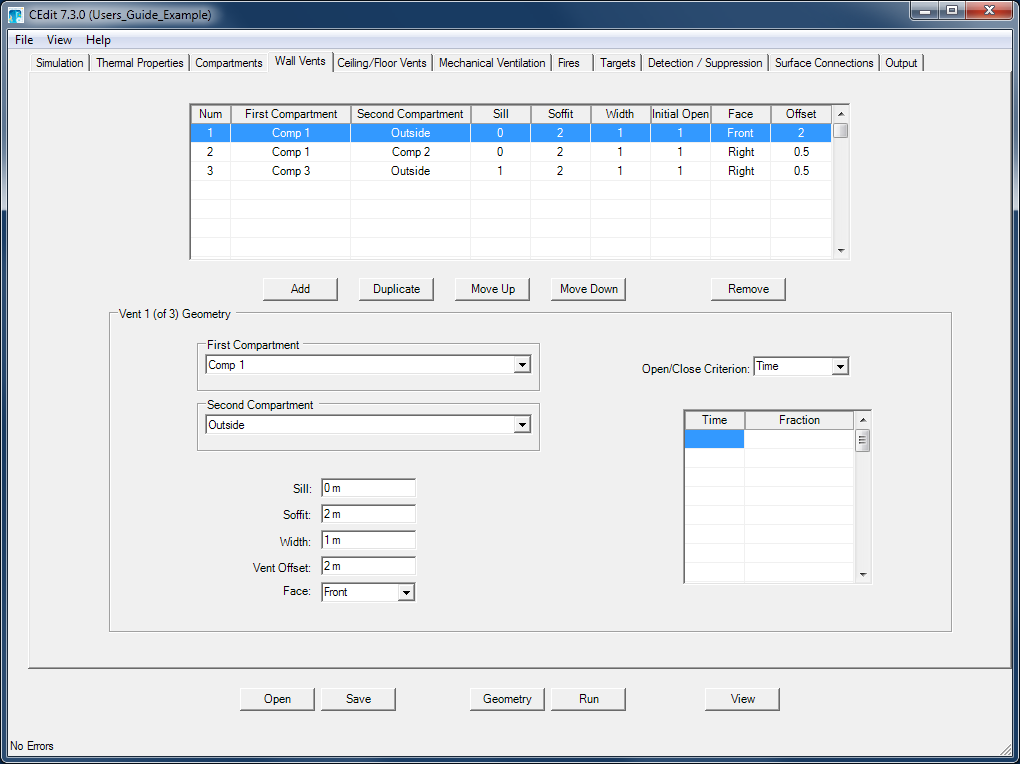
\includegraphics[width=6.5in]{FIGURES/Natural_Flow_Tab}
\caption[The CFAST Wall Vents Tab]{The CFAST Wall Vents Tab.}
\end{center}
\end{figure}

Wall vents are doors or windows that connect compartments that physically overlap in elevation, or that connect to the outside. Horizontal flow connections may also be used to account for leakage between compartments or to the outdoors.

\begin{description}
\item[ID] The selected name must be unique (i.e., not the same as another vent in the same simulation).
\item[First Compartment] First of the two compartments connected by a door or window. All specifications of the vent are made relative to the floor of the first compartment.
\item[Second Compartment] Second of the two compartments connected by a door or window.
\item[Bottom] (default units: m, default value: 0 m): Position of the bottom of the opening relative to the floor of the first compartment.
\item[Height] (default units: m, default value: 0 m): Height of the opening relative to the bottom of the opening.
\item[Width] (default units: m, default value: 0 m): The width of the opening.
\item[Vent Offset] (default units: m, default value: 0 m): For visualization only, the horizontal distance between the near edge of the vent and the origin of the axis defined by the selected face (below) in the first compartment.
\item[Face] The wall on which the vent is positioned.  Choices are Front, Rear, Right, Left and are relative to the X-Z plane (Front and Rear faces are parallel to the X-axis; left and right are parallel to the Y-axis).
\end{description}

Vents in CFAST can be opened or closed at user-specified times or by a user-specified target's surface temperature or incident heat flux. For time-based opening changes, the inputs are a series of time points and associated opening fractions from 0 (fully closed) to 1 (fully open).

\begin{description}
\item[Time] (default units: s, default values: 0 s): Time during the simulation at which to begin or end a change in the open fraction.
\item[Fraction] (default value: 1, fully open): Fraction between 0 and 1 of the vent width to indicate the vent is closed, partially-open, or fully-open as the associated time point.
\end{description}

For condition-based opening changes, the inputs specify an associated target, trigger value, and vent opening fractions before and after the trigger value has been reached.

\begin{description}
\item[Open/Close Criterion] The time of ignition can be controlled by a user-specified time, or by a user-specified target's surface temperature or incident heat flux.
\item[Set Point] The critical value at which the vent opening change will occur. If it is less than or equal to zero, the default value of zero is taken.
\item[Trigger Target] User-specified target used to calculate surface temperature or incident heat flux to trigger a vent opening change. Target placement is specified by the user as part of the associated target definition.
\item[Pre-Activation Fraction] (default value: 1, fully open): Fraction between 0 and 1 of the vent width to indicate the vent is partially open at the start of the simulation.
\item[Post-Activation Fraction] (default value: 1, fully open): Opening fraction at the end of the simulation. The transition from the pre-activation fraction to the post-activation value is assumed to occur over one second beginning when the specified set point value is reached.
\end{description}

\graybox{CFAST assumes a linear transition between time points. If the initial time specified for a time-changing opening fraction is non-zero, the vent is assumed to be open at the initial value of the open fraction from the beginning of the simulation up to and including the time associated with the initial value of the opening fraction. If the final value of the opening fraction is less than the total simulation time, the vent is assumed to be open at the final value of the opening fraction from and including the time associated with the final value of the opening fraction until the end of the simulation.}




\subsection{Ceiling/Floor Vents}
\label{info:VENT2}
\begin{figure}[h!]
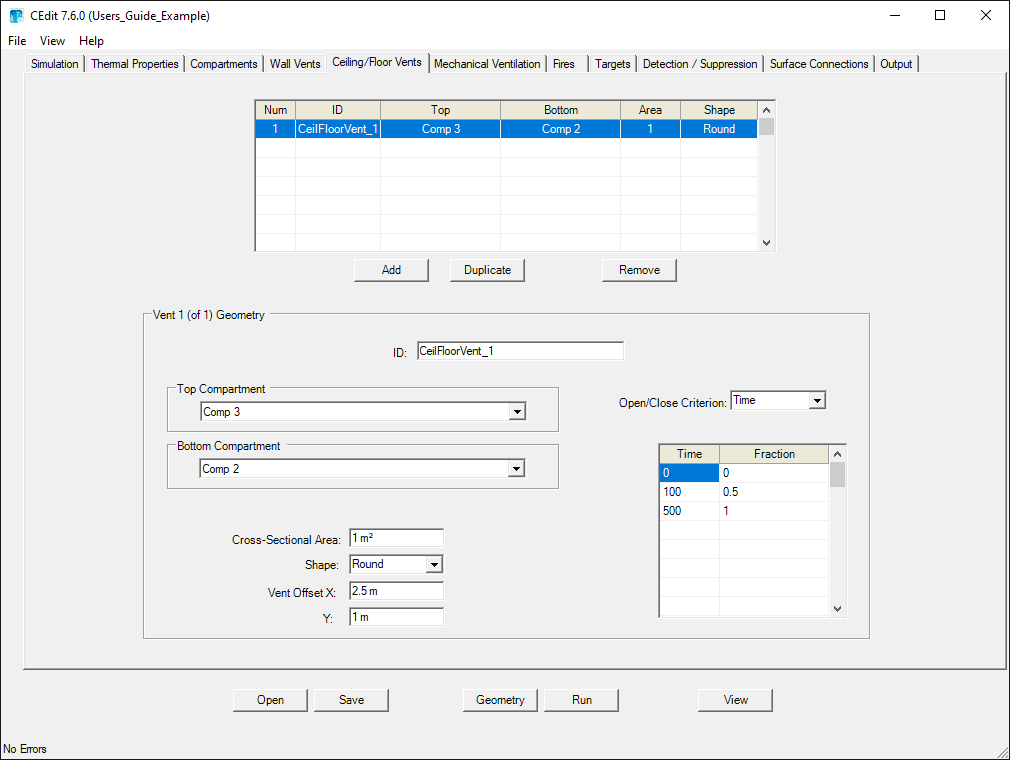
\includegraphics[width=6.5in]{FIGURES/Vertical_Flow_Tab}
\caption[The CFAST Ceiling/Floor Vents Tab]{The CFAST Ceiling/Floor Vents Tab.}
\end{figure}

Examples of these openings are scuddles in a ship, or a hole in the roof of a residence. Connections can exist between compartments or between a compartment and the outdoors. Combined buoyancy and pressure-driven flow through a vertical flow vent is possible when the connected spaces adjacent to the vent are filled with gases of different density in an unstable configuration, with the density of the top space greater than that of the bottom space. With a moderate cross-vent pressure difference, the instability leads to a bi-directional flow between the two spaces. For relatively large cross-vent pressure difference the flow through the vent is unidirectional.

\begin{description}
\item[ID] The selected name must be unique (i.e., not the same as another vent in the same simulation).
\item[Top Compartment] Compartment where the vent is in the floor
\item[Bottom Compartment] The adjacent compartment where the vent is in the ceiling.
\label{Ceil Cross-sectional Area}
\item[Cross-sectional Area] (default units: m$^2$, default value: 0 m$^2$)
\label{Ceil Shape}
\item[Shape] The shape factor changes the calculation of the effective diameter of the vent and flow coefficients for flow through the vent.
\item[Vent Offset] (default units: m, default value: 0 m): For visualization only, the horizontal distances between the center of the vent and the origin of the X and Y axes in the upper compartment. See figure \ref{fig:compartment_positioning} for axis position conventions in CFAST.
\end{description}

Vents in CFAST can be opened or closed at user-specified times or by a user-specified target's surface temperature or incident heat flux. For time-based opening changes, the inputs are a series of time points and associated opening fractions from 0 (fully closed) to 1 (fully open).

\begin{description}
\item[Time] (default units: s, default value: 0 s): Time during the simulation at which to begin or end a change in the open fraction.
\item[Fraction] (default value: 1, fully open): Fraction between 0 and 1 of the vent width to indicate the vent is closed, partially-open, or fully-open as the associated time point.
\end{description}

For condition-based opening changes, the inputs specify an associated target, trigger value, and vent opening fractions before and after the trigger value has been reached.

\begin{description}
\item[Open/Close Criterion] The time of ignition can be controlled by a user-specified time, or by a user-specified target's surface temperature or incident heat flux.
\item[Set Point] The critical value at which the vent opening change will occur. If it is less than or equal to zero, the default value of zero is taken.
\item[Trigger Target] User-specified target used to calculate surface temperature or incident heat flux to trigger a vent opening change. Target placement is specified by the user as part of the associated target definition.
\item[Pre-Activation Fraction] (default value: 1, fully open): Fraction between 0 and 1 of the vent width to indicate the vent is partially open at the start of the simulation.
\item[Post-Activation Fraction] (default value: 1, fully open): Opening fraction at the end of the simulation. The transition from the pre-activation fraction to the post-activation fraction is assumed to occur over one second beginning when the specified set point value is reached.
\end{description}

\graybox{CFAST assumes a linear transition between time points. If the initial time specified for a time-changing opening fraction is non-zero, the vent is assumed to be open at the initial value of the open fraction from the beginning of the simulation up to and including the time associated with the initial value of the opening fraction. If the final value of the opening fraction is less than the total simulation time, the vent is assumed to be open at the final value of the opening fraction from and including the time associated with the final value of the opening fraction until the end of the simulation.

CFAST allows only a single ceiling/floor connection between any pair of compartments included in a simulation because the empirical correlation governing the flow was developed using only a single opening between connected compartments.

Vertical connections can only be created between compartments that could be physically stacked based on specified floor and ceiling elevations for the compartments.  Some overlap between the absolute floor height of one compartment and the absolute ceiling height of another compartment is allowed.  However, whether the compartments are stacked or overlap somewhat, the ceiling/floor absolute elevations must be within 0.01 m of each other. The check is not done when the connection is to the outside.}




\section{Mechanical Ventilation}
\begin{figure}[h!]
\begin{center}
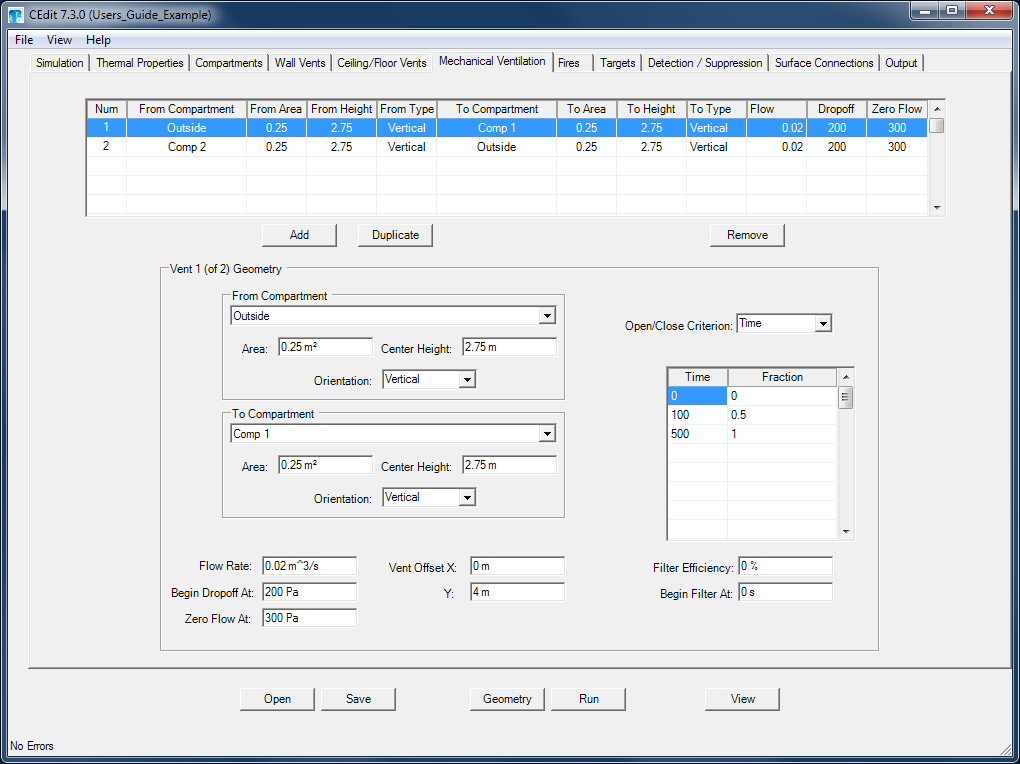
\includegraphics[width=6.5in]{FIGURES/Mechanical_Vent_Tab}
\caption[The CFAST Mechanical Vents Tab]{The CFAST Mechanical Vents Tab.}
\end{center}
\end{figure}

Fan-duct systems are commonly used in buildings for heating, ventilation, air conditioning, pressurization, and exhaust. Generally, systems that maintain comfortable conditions have either one or two fans.  Residences often have a system with a single fan. Further information about these systems is presented in  Klote and Milke \cite{Klote:2002} and the  \textit{Handbook of Smoke Control Engineering} \cite{Klote:2012}.

CFAST models mechanical ventilation in terms of user-specified volume flows at various points in the compartment. The model does not include duct work or fan curves, and thus mechanical ventilation connections are simply described by the connections to the two compartments and a fan whose throughput is a constant volumetric flow up to a user-specified pressure drop across the fan, dropping to zero at high backwards pressure on the fan.

\subsection{Connections to Compartments}
\label{info:VENT3}
\begin{description}
\item[ID]  The selected name must be unique (i.e., not the same as another mechanical ventilation system in the same simulation).
\item[First Compartment] The compartment from which the fan flow originates.
\item[Second Compartment] The compartment to which the fan flow terminates.
\item[Area] (default units: m$^2$, default value: 0 m$^2$): Cross-sectional area of the opening.
\label{Mech Height}
\item[Center Height] (default units: m, default value: 0 m): Height of the midpoint of the duct opening above the floor.
\item[Orientation] (default vertical) A horizontal diffuser implies vertical flow through the ceiling or floor of the compartment.  A vertical diffuser implies horizontal flow through a wall of the compartment.
\item[Vent Offset] (default units: m, Default value: 0 m): For visualization only, the horizontal distances between the center of the vent and the origin of the X and Y axes in the first compartment. See figure \ref{fig:compartment_positioning} for axis position conventions in CFAST.
\end{description}

Vents in CFAST can be opened or closed at user-specified times or by a user-specified target's surface temperature or incident heat flux. For time-based opening changes, the inputs are a series of time points and associated opening fractions from 0 (fully closed) to 1 (fully open).

\begin{description}
\item[Time] (default units: s, default values: 0 s): Time during the simulation at which to begin or end a change in the open fraction.
\item[Fraction] (default value: 1, fully open): Fraction between 0 and 1 of the vent width to indicate the vent is closed, partially-open, or fully-open as the associated time point.
\end{description}

\graybox{CFAST assumes a linear transition between time points. If the initial time specified for a time-changing opening fraction is non-zero, the vent is assumed to be open at the initial value of the open fraction from the beginning of the simulation up to and including the time associated with the initial value of the opening fraction. If the final value of the opening fraction is less than the total simulation time, the vent is assumed to be open at the final value of the opening fraction from and including the time associated with the final value of the opening fraction until the end of the simulation.}

For condition-based opening changes, the inputs specify an associated target, trigger value, and vent opening fractions before and after the trigger value has been reached.

\begin{description}
\item[Open/Close Criterion] The time of ignition can be controlled by a user-specified time, or by a user-specified target's surface temperature or incident heat flux.
\item[Set Point] The critical value at which the vent opening change will occur. If it is less than or equal to zero, the default value of zero is taken.
\item[Trigger Target] User-specified target used to calculate surface temperature or incident heat flux to trigger a vent opening change. Target is placement is specified by the user as part of the associated target definition.
\item[Pre-Activation Fraction] (default value: 1, fully open): Fraction between 0 and 1 of the vent width to indicate the vent is partially open at the start of the simulation.
\item[Post-Activation Fraction] (default value: 1, fully open): Opening fraction at the end of the simulation. The transition from the pre-activation fraction to the post-activation fraction is assumed to occur over one second beginning when the specified set point value is reached.
\end{description}




\subsection{Fans}
\label{info:VENT4}
CFAST does not include provisions for reverse flow through a fan, or a fan curve. Rather, you may specify a pressure above which the flow linearly decreases to zero.
\begin{description}
\label{Mech Flow Rate}
\item[Flow Rate] (default units: m$^3$/s, default value: 0 m$^3$/s): Constant flow rate of the fan.
\label{Mech Begin Drop Off Pressure}
\item[Begin Drop Off Pressure] (default units: Pa, default value: 200 Pa): Above this pressure, the flow begins a drop-off to zero. A hyperbolic tangent function is used to ensure a smooth transition from full flow at the ``Begin Drop Off Pressure'' to zero flow at the ``Zero Flow Pressure''.
\label{Mech Zero Flow Pressure}
\item[Zero Flow Pressure] (default units: Pa, default value: 300 Pa): The pressure above which the flow is zero.
\end{description}




\subsection{Filtering}
\label{info:VENT5}
For mechanical vents, there are two species that can be filtered out of the gas flow: soot and the user-defined trace species. Filters are applied only to fan openings. The fan must have been defined before the filter can be applied. Initially filtering is off.
\begin{description}
\label{Mech Filter Efficiency}
\item[Filter Efficiency] (default units:~\%, default value: 0\%): Flow through mechanical vents may include filtering that removes a user-specified portion of soot and trace species mass from the flow through the vent.  By default, there is no filtering applied; that is, all of the soot and trace species mass in the vent flow is passed through the vent. Within the user interface, this is specified as a filter efficiency of 0~\%.  If desired, you may specify the fraction of the soot and trace species mass to be removed as a percentage.
\label{Mech Begin Filtering At Time}
\item[Begin Filtering At Time] (default units: s, default value: 0 s): Time during the simulation at which the mechanical vent filtering begins.
\end{description}

\graybox{If the simulation includes mechanical ventilation filtering, care should be taken in choosing trace species production rates to insure the production rate is small compared to the total pyrolysis rate since the filtering removes mass from the system.  This will better allow appropriate conservation of mass in the solution of the system of differential equation.  For large production rates of trace species, scaling factors can be used (e.g., divide by 1000) for the trace species production rate to reduce the relative magnitude compared to the pyrolysis rate.  For analysis, the resulting trace species in compartments and filters can be converted back to original units multiplying by the scaling factor used.}






\chapter{Fires}
A fire in CFAST is specified via a time-dependent heat release rate (HRR). The specified heat of combustion is used to calculate the mass loss rate of fuel, from which the production rate of combustion products can be calculated using specified product yields. The heat release and the corresponding product generation rates go to zero when the lower oxygen limit is reached, and are replaced by the appropriate production rate of unburned fuel gas which is transported from zone to zone until there is sufficient oxygen and a high enough temperature to support combustion.

The model can simulate multiple fires in one or more compartments. These fires are treated as totally separate entities, with no interaction of the plumes. These fires can be ignited at a prescribed time, or when a corresponding target (see Chapter~\ref{chapter:targets}) reaches a specified temperature or heat flux.

The combustion model is defined by the following one-step reaction:
\begin{eqnarray}
   \mathrm{C_{n_\C}H_{n_H}O_{n_O}N_{n_N}Cl_{n_{Cl}}} &+&  \nu_\OTWO \, \mathrm{O_2}  \rightarrow  \nonumber \\[.1in]
   \nu_\COTWO \, \mathrm{CO_2} &+& \nu_\HTWOO \, \mathrm{H_2O} \; + \; \nu_\CO \, \mathrm{CO} \; + \; \nu_\So \, \mathrm{Soot} \; + \; \nu_\HCl \mathrm{HCl} \; + \; \nu_\HCN \mathrm{HCN} \label{stoich}
\end{eqnarray}
It is assumed that all the nitrogen and chlorine in the fuel are converted to HCN and HCl.

\begin{figure}[h!]
\begin{center}
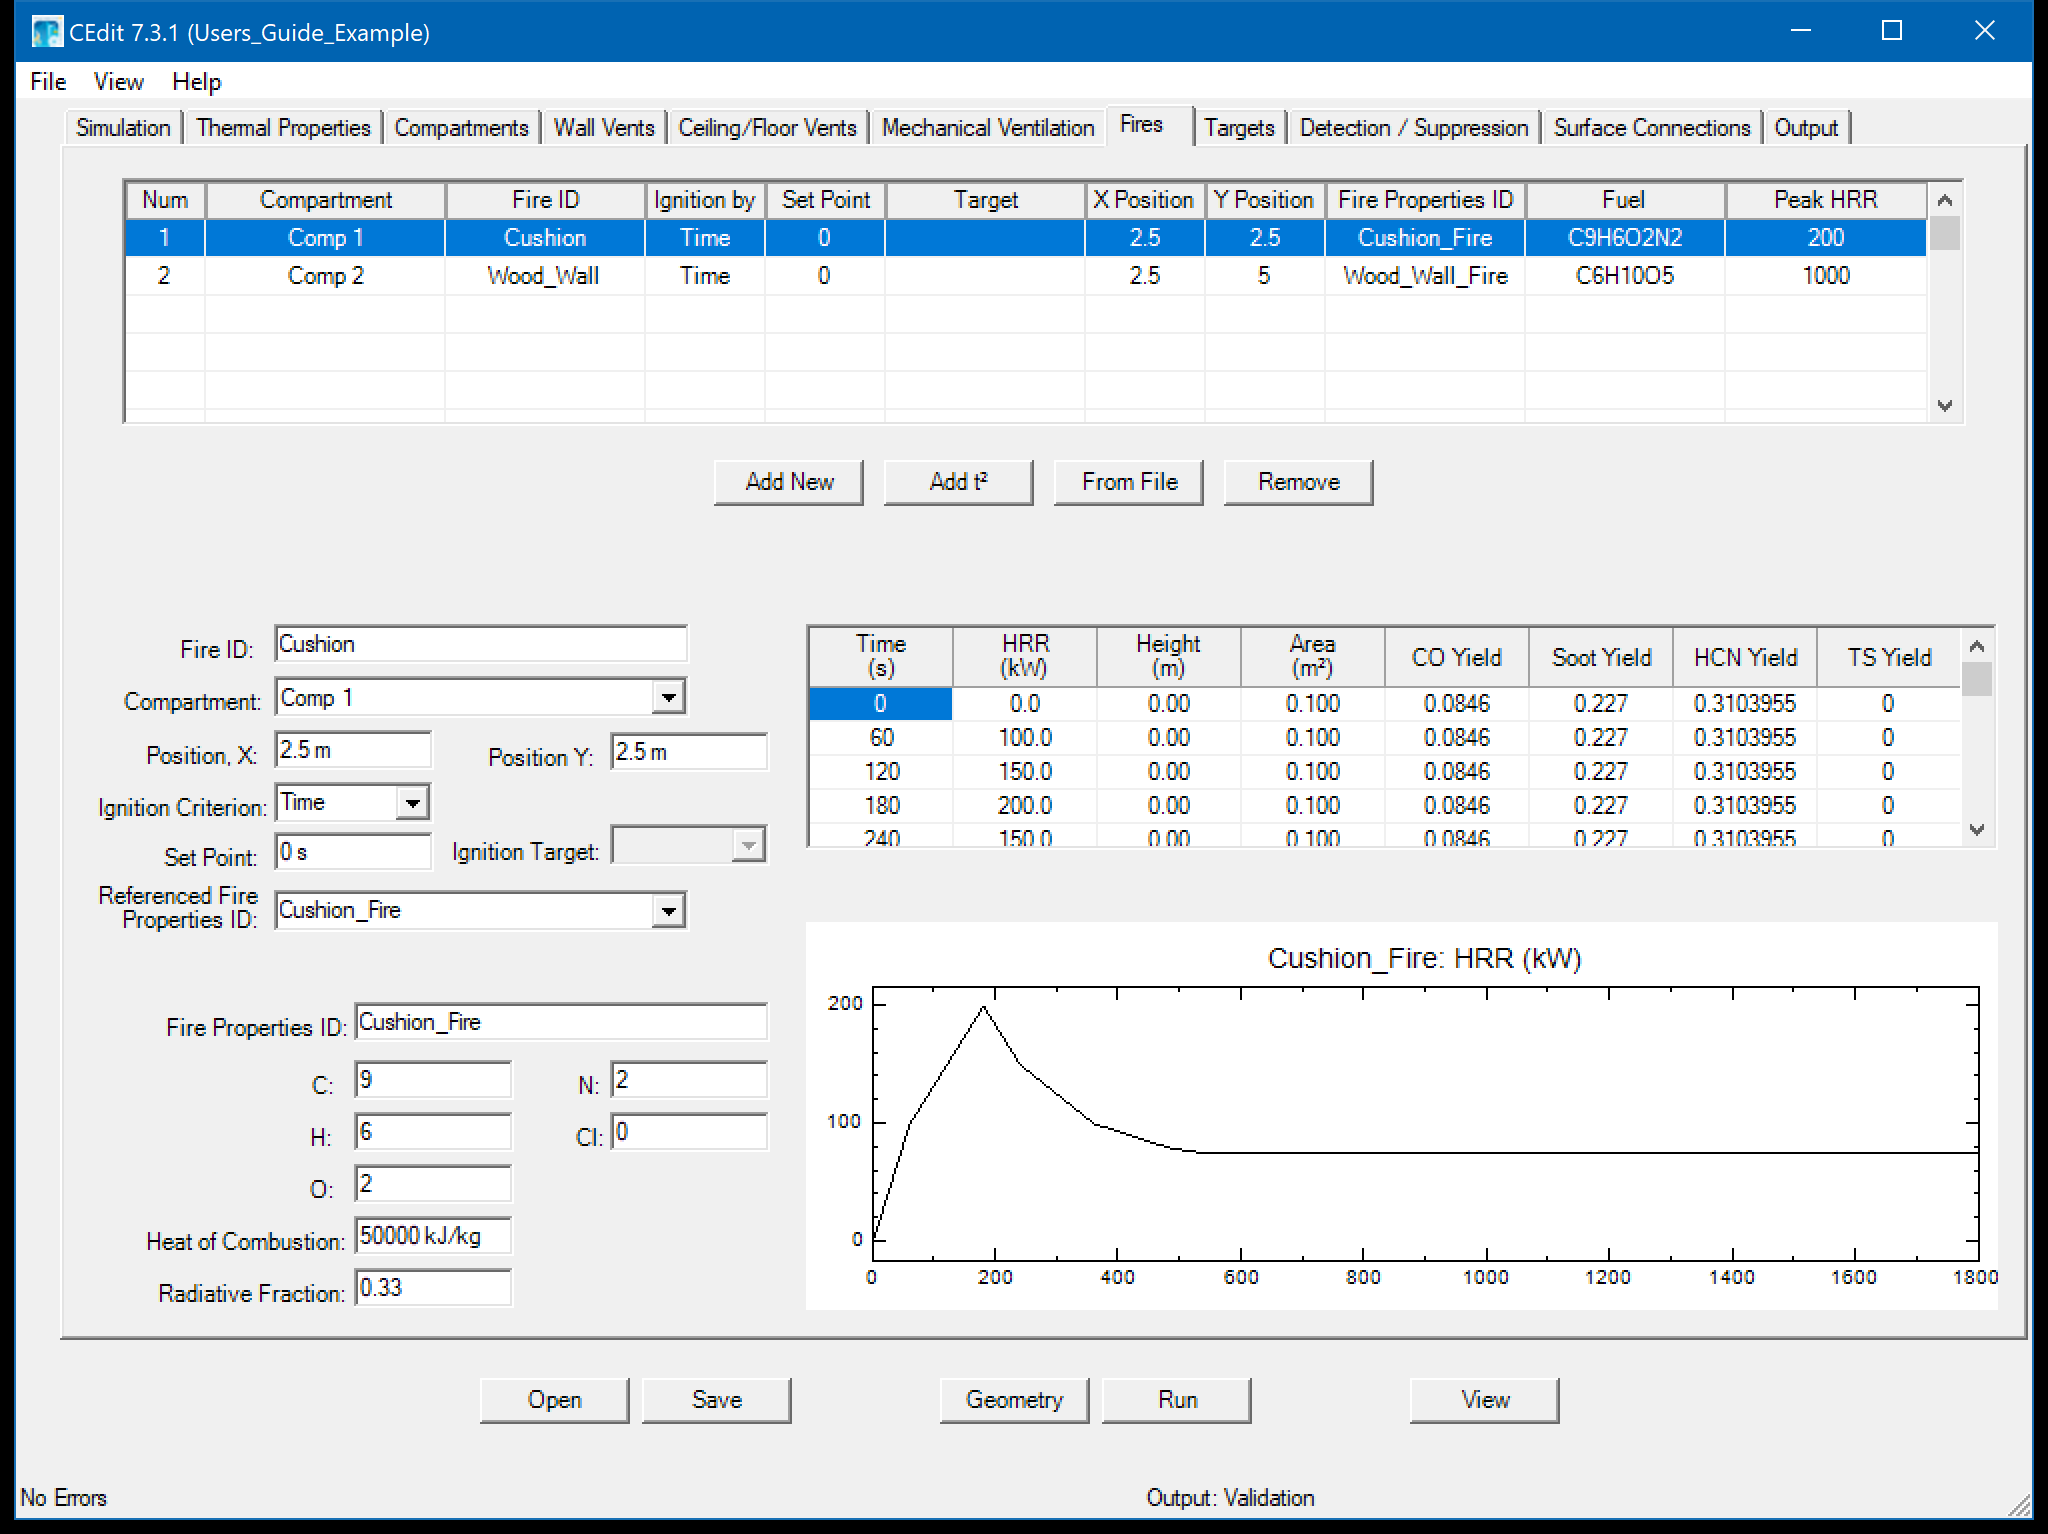
\includegraphics[width=6.5in]{FIGURES/Fire_Tab}
\caption[The CFAST Fires Tab]{The CFAST Fires Tab.}
\end{center}
\end{figure}


\section{Adding Fires}
\label{info:FIRE}
\label{sec:fire_inputs}
Fires in CFAST are defined in two parts: a ``Fire Definition'' that specifies the fuel composition, heat release rate, and species yields for the fire, and a ``Fire Instance'' that specifies the placement of a defined fire within a compartment in the simulation. A single fire definition may be associated with more than one fire instance in a simulation if desired.

For a new fire , click on the {\bf Add New} button or {\bf Add t$^2$} buttons within the fire definition block of inputs. The latter is useful because it has predefined quadratic growth rate options that are commonly used in fire analyses. See Section~\ref{tsq} for details. For each fire instance, specify the following properties:
\begin{description}
\item[Fire ID] The selected name must be unique (i.e., not the same as another fire instance in the same simulation).
\item[Compartment] Name of the compartment where the fire occurs.
\item[Position X, Y] (default units: m, default value: compartment center): Position of the center of the base of the fire relative to the front left corner of the compartment.
\item[Ignition Criterion] The time of ignition can be controlled by a user-specified time, or by a user-specified target's surface temperature or incident heat flux.
\item[Set Point] The critical value at which ignition will occur. If it is less than or equal to zero, the default value of zero is taken.
\item[Ignition Target] User-specified target used to calculate surface temperature or incident heat flux to ignite fire. Target is typically placed at the base of the fire to be ignited.
\item[Referenced Fire] the name of the associated fire definition for this fire instance can be selected from a list of fire definitions. A fire definition must exist before it can be selected.
\end{description}

Each instance of a fire can be unique fires with different chemical composition and time-dependent fire properties. Alternatively, two or more fires can reference the same set of fire properties. The following parameters define the composition and burning properties of the fire.
\begin{description}
\item[Fire Properties ID] The selected name must be unique (i.e., not the same as another fire definition in the same simulation). IDs for fire definitions can be the same as ones for fire instances.
\item[C, H, O, N, Cl] The number of each atom in the fuel molecule. Burning fuels in CFAST are assumed to be hydrocarbon fuels that contain at least carbon and hydrogen and optionally oxygen, nitrogen, and chlorine. All of the specified nitrogen and chlorine is assumed to completely react to form HCN and HCl.
\item[Heat of Combustion] (default units: kJ/kg, default value: 50000 kJ/kg): The energy released per unit mass of fuel consumed.
\item[Radiative Fraction] (default units: none, default value: 0.35): The fraction of the combustion energy that is emitted in the form of thermal radiation. Values for various fuels are suggested by Beyler~\cite{Beyler2:SFPE}.
\end{description}



\section{Time-Dependent Properties}
\label{info:FIRE2}
Following is a list of fire properties that can be specified as a function of time. The properties are linearly interpolated between specified points. If the simulation time is longer than the total duration of the fire, the final values specified for the fire are continued until the end of the simulation. Normal copy (Ctrl-C), cut (Ctrl-X), and paste (Ctrl-V) keyboard shortcuts work for data editing. In addition, Alt-Insert will insert a complete row above the currently-selected row in the spreadsheet and Alt-Delete will delete the current row in the spreadsheet.
\begin{description}
\item[Time] (default units: s, default values: none): Time from ignition.
\item[HRR] (default units: kW, default values: none): Heat release rate of the fire.
\item[Height] (default units: m, default values: 0 m): Height of the base of the fire.
\item[Area] (default units: m$^2$, default values: calculated from heat release rate such that the fire Froude number is unity\footnote{The Fire Froude Number, $\dot{Q}^*$, is defined as $\dot{Q}^* = \frac{\dot{Q}}{\rho_\infty c_p T_\infty \sqrt{gD} D^2}$. It is essentially the ratio of the fuel gas exit velocity and the buoyancy-induced plume velocity. Jet fires are characterized by large Froude numbers. Typical accidental fires have a Froude number near unity.}): Area of the base of the fire. The plume correlations used in CFAST generally regard the base to be circular. Do not set this value to zero because it is used in the various plume correlations.
\item[CO Yield] (default units: kg/kg, default value: 0 kg/kg): Mass of CO produced per unit mass of fuel consumed.
\item[Soot Yield] (default units: kg/kg, default value: 0 kg/kg): Mass of soot produced per unit mass of fuel consumed.
%Should this still be there if all the N2 in the fuel is assumed to go to HCN.
\item[HCN Yield] (default units: kg/kg, default value: 0 kg/kg): Mass of hydrogen cyanide produced per unit mass of fuel consumed.
\item[TS Yield] (default units: kg/kg, default value: 0 kg/kg): Mass of user-defined trace species per unit mass of fuel consumed. The trace species is transported along with the other products of combustion, but is assumed not to take part in the combustion reaction and is assumed not to be a significant source of overall mass for the system mass balance. This implies that the production rate of trace species specified should be small.
\end{description}


\section{Special Topic: t-Squared Fires}
\label{tsq}
Use the `Add t$^2$' button to create a new fire with a heat release rate that grows as a function of the time squared~\cite{Schifiliti:2002}:
\be
   \dQ(t) = \dQ_{\rm peak} \; \left( \frac{t}{t_{\rm peak}} \right)^2
\ee

\begin{figure}[h!]
\begin{center}
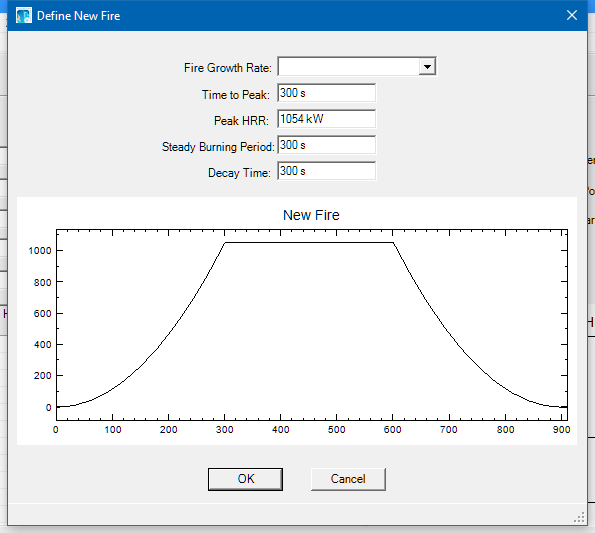
\includegraphics[width=5in]{FIGURES/Create_t2}
\caption[Inserting T-squared Fires in CFAST]{Inserting T-squared Fires in CFAST.}
\end{center}
\end{figure}

\begin{description}
\item[Fire Growth Rate] A set of specific t-squared fires labeled slow, medium, fast, or ultra-fast such that the fire reaches 1054~kW (1000~BTU/s) in 600~s, 300~s, 150~s, and 75~s.  A custom selection allows you to define any growth or decay rate desired.
\item[Time to Peak] (default units: s, default value: 300 s): The time for the fire to reach the peak HRR.
\item[Peak HRR] (default units: kW, default value: 1054 kW): The peak heat release rate of the t-squared fire.
\item[Steady Burning Period] (default units: s, default value: 300 s): Duration of time that the fire continues burning at the rate specified by the peak HRR.
\item[Decay Time] (default units: s, default value, 300 s): Duration of time for the fire to decay back to a zero value.  Decay follows the inverse of the t-squared growth rate.
\end{description}

%Where is the getting fire definitions from files?






\chapter{Measurement and Fire Protection Devices}
\label{info:DEVC}
\section{Targets}
\label{chapter:targets}

A target is any object in the simulation that can heat up via radiative and convective heat transfer. The heat conduction into the target is performed via a one-dimensional calculation in either cartesian or cylindrical coordinates.

\begin{figure}[h!]
\begin{center}
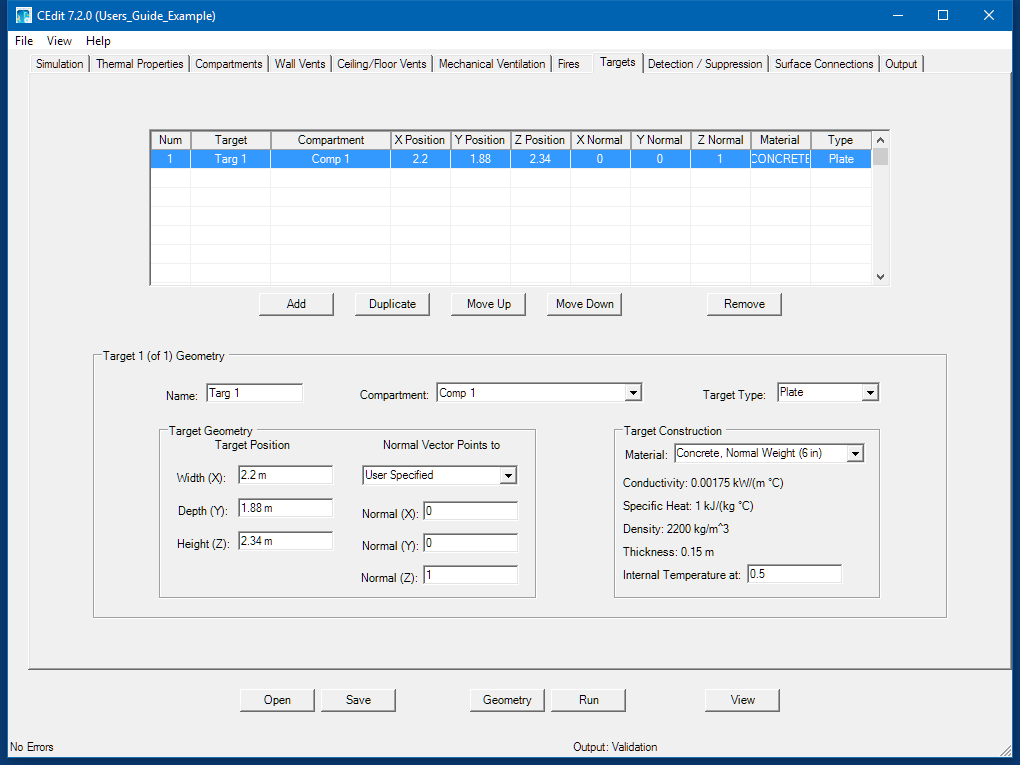
\includegraphics[width=6.5in]{FIGURES/Target_Tab}
\caption[The CFAST Targets Tab]{The CFAST Targets Tab.}
\end{center}
\end{figure}

\begin{description}
\item[ID] The selected name must be unique (i.e., not the same as another target in the same simulation).

\item[Compartment] The compartment in which the target is located.

\item[Target Type] Specify Plate, or Cylindrical.  For plate targets, CFAST solves a partial differential equation in cartesian coordinates, and for cylindrical targets, a partial differential equation in cylindrical coordinates.

\item[Width (X)] (default units: m): Distance from the left wall of the target compartment.

\item[Depth (Y)] (default units: m): Distance from the front wall of the target compartment.

\item[Height (Z)] (default units: m): Height of the target above the floor.

\item[Normal Vector (X,Y,Z)]: specifies a vector of unit length perpendicular to the exposed surface of the target. For example, the vector (-1,0,0) indicates that the target is facing the left wall. The vector (0,0,1) is facing the ceiling.

\item[Material] What the target is made of. Any existing material in the list of thermal properties may be used here. There can be only one material per target.

%What happens to interanl temperatrue when type is cylindrical
\item[Internal Temperature] (default units: none, default value: 0.5): For each target, CFAST calculates the internal temperature at a number of node points within the target. By default, the reported internal temperature (in the printed and spreadsheet output) is the temperature at the center of the target, e.g., equidistant from the front and back faces of the target. This input allows the user to override this default position. The input represents the position as a fraction of the thickness from the front surface to the back surface of the material.
\end{description}

\graybox{
If the target is only needed to report the local gas temperature, which may include the plume or ceiling jet, then you may specify arbitrary properties and normal vector. The output spreadsheet file includes the local gas temperature in addition to the target temperature.

The normal vectors in the $x$, $y$, and $z$ directions from a target at [$x$, $y$, $z$] to a location [$x_L$, $y_L$, $z_L$] are:
\begin{eqnarray}
x_N &=& \frac{x_L - x}{\sqrt{\brackets{x_L - x}^2 + \brackets{y_L - y}^2 + \brackets{z_L - z}^2}} \\[.1in]
y_N &=& \frac{y_L - y}{\sqrt{\brackets{x_L - x}^2 + \brackets{y_L - y}^2 + \brackets{z_L - z}^2}} \\[.1in]
z_N &=& \frac{z_L - z}{\sqrt{\brackets{x_L - x}^2 + \brackets{y_L - y}^2 + \brackets{z_L - z}^2}}
\end{eqnarray}
}




\section{Sprinklers and Detectors}
\label{info:DEVC2}
Sprinklers and detectors are both considered detection devices by the CFAST model and are handled using the same inputs.  Detection is based upon heat transfer to the detector. Fire suppression by a user-specified water spray begins once the associated detection device is activated.


\begin{figure}[h!]
\begin{center}
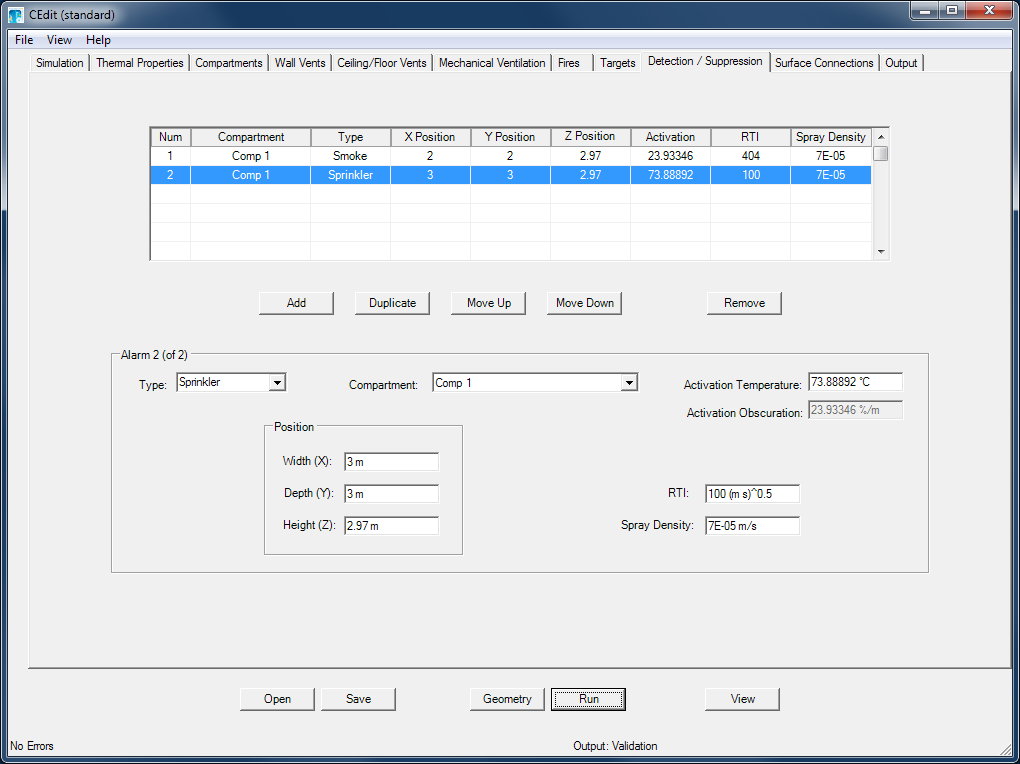
\includegraphics[width=6.5in]{FIGURES/Detector_Tab}
\caption[The CFAST Detection/Suppression Tab]{The CFAST Detection/Suppression Tab.}
\end{center}
\end{figure}

\begin{description}
\item[ID]  The selected name must be unique (i.e., not the same as another sprinkler or detector in the same simulation).

\item[Type] type of detector, select smoke detector, heat detector, or sprinkler.

\item[Compartment] the compartment in which the detector or sprinkler is located.

\item[Activation Temperature] (default units: \degc, default value: dependent on type): the temperature at or above which the detector link activates.

\item[Activation Obscuration] (default units: \%/m, default value: 23.93 \%/m (8 \%/ft)): the obscuration at or above which the detector link activates.

\item[Width (X)] Position (default units: m, default value: none): position of the object as a distance from the left wall of the compartment (X direction).

\item[Depth (Y)] Position (default units: m, default value: none): position of the detector or sprinkler as a distance from the front wall of the compartment (Y direction).

\item[Height (Z)] Position (default units: m, default value: none): position of the object as a distance from the floor of the compartment (Z direction).

\item[RTI] (default units: (m$\cdot$s)$^{1/2}$, default value: none): the Response Time Index (RTI) for the sprinkler or detection device.

\item[Spray Density] (default units: m/s, default value: none): the amount of water dispersed by a sprinkler.  The units for spray density are length/time, derived by dividing the volumetric flow rate by the spray area. The suppression calculation is based upon an experimental correlation by Evans~\cite{Evans:1993}.
\end{description}

\graybox{
Care should be taken when specifying detectors to activate based on smoke obscuration since the only calculation included in CFAST is a simple two-zone calculation of soot concentration that does not include the impact of an initial ceiling layer as is done for temperature-based calculations. Often, the activation of smoke alarms is simulated with a temperature-based criterion (in CFAST as a heat alarm), typically in the range of 5~\degc to 10~\degc above ambient. Davis and Notarianni  studied the activation of heat and smoke alarms in small and large compartments \cite{Davis:1996}. They conclude that a temperature rise of approximately 5~\degc corresponded to activation of ionization alarms for a range of fire sources and ceiling heights. The Nuclear Regulatory Commission includes a default value of 10~\degc with an RTI value of 5 (m$\cdot$s)$^{1/2}$ in NUREG-1805 \cite{NRCNUREG1805}. \\

Several cautions should be observed when using estimates of sprinkler suppression within the model: 1)~The first sprinkler activated controls the effect of the sprinkler on the heat release rate of the fire.  Subsequent sprinklers which may activate have no additional effect on the fire simulation. 2)~The fire suppression algorithm assumes the effect of the sprinkler is solely to reduce the heat release rate of the fire. Any effects of the sprinkler spray on gas temperatures or mixing within the compartment are ignored. 3)~The sprinkler always reduces the heat release rate of the fire. The ability of a fire to overwhelm an under-designed sprinkler is not modeled. 4) Since the dynamics of the sprinkler and direct effects of the spray on gas temperatures and velocities are not modeled, calculated times of activation of secondary sprinklers and / or detectors after the first sprinkler is activated should not be modeled since the impact of the first sprinkler on the activation of additional sprinklers is not included in the CFAST model.}




\chapter{Surface Connections}
\label{info:CONN}
\begin{figure}[h!]
\begin{center}
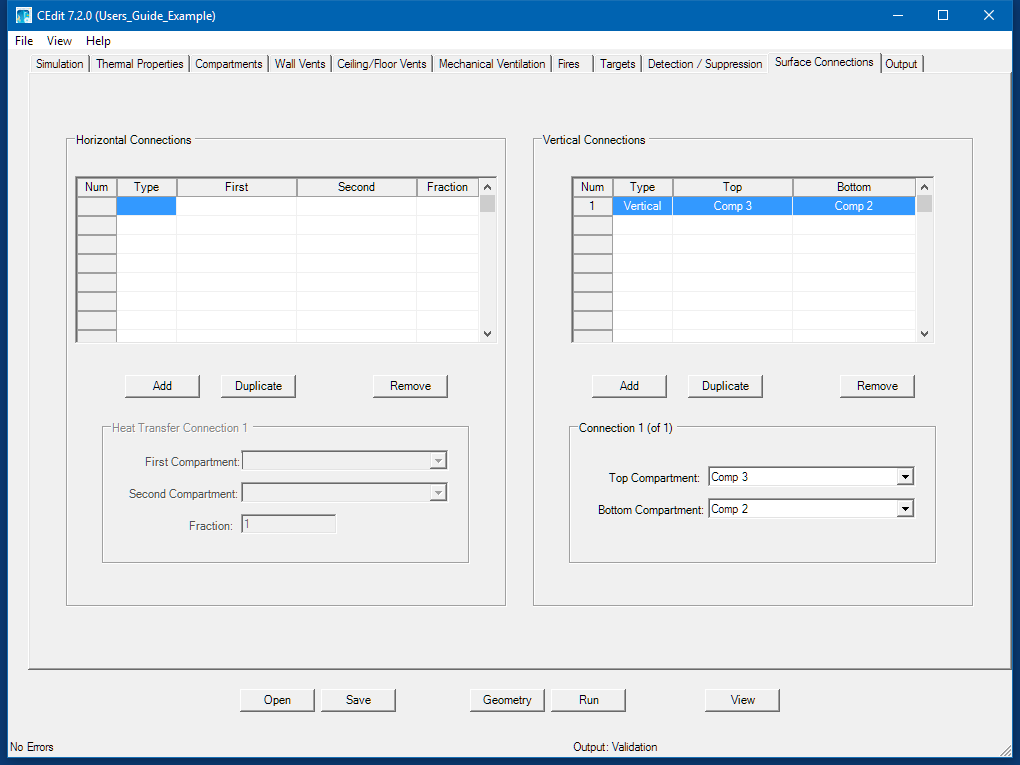
\includegraphics[width=6.5in]{FIGURES/Surface_Connection_Tab}
\caption[The CFAST Surface Connections Tab]{The CFAST Surface Connections Tab.}
\end{center}
\end{figure}

The Surface Connections page allows the user to define heat transfer between compartments in a simulation. Energy can be transferred from compartment to compartment through solid boundaries (walls, ceilings and floors) by means of conduction. The heat transfer between connected compartments is modeled by setting the boundary condition for the outside surface of a compartment to the temperature of the outside surface of the  connected compartment.   As before, temperatures are determined by the solver so that the heat flux striking the wall surface (both interior and exterior) is consistent with the temperature gradient at that surface.

\begin{description}
\item[First Compartment] First of the compartments whose walls are connected for horizontal heat transfer.

\item[Second Compartment] Second of the compartments whose walls are connected for horizontal heat transfer.

\item[Fraction] Specifies the fraction of the vertical surface areas of the compartments which are connected. The fraction specifies the fraction of the vertical surface area of the first compartment that connects the first and second compartment pair.

\item[Top Compartment] The top or first of the two compartments to be connected by a vertical heat transfer connection. The connection is through the floor of this compartment.

\item[Bottom Compartment] The bottom or second of the two compartments to be connected by a vertical heat transfer connection. The connection is through the ceiling of this compartment.
\end{description}

\graybox{Consider two compartments that share a single wall. Both compartments are 1 m x 1 m x 1 m in size. The resulting horizontal heat transfer connections would be 0.25 for both compartments since they share 1 m$^2$ of a total wall surface of 4 m$^2$. If the compartments are of different size, then the fraction would be different for the two directions. For example, if compartment 1 is 1 m x 1 m x 1 m and compartment 2 is 2 m x 2 m x 2 m, then the connection from 1$>$2 is 0.25 and the connection from 2$>$1 is 0.125.

For horizontal heat transfer, you must include a connection for each compartment. For example, for a connection between compartment 1 and compartment 2, you must include a connection from 1 to 2 AND a connection from 2 to 1.  For consistency, the fraction for each compartment needs to specify equal areas in the two compartments.  Fractions for connections should add to unity.  An error is generated if the fractions for a compartment add to greater than unity. If the fractions for a compartment add to less than unity, the remaining surface area will be assigned to be connected to the outdoors.}




\chapter{Visualization}

Calculated results from a CFAST simulation can be visualized using Smokeview \cite{Smokeview_Users_Guide_6}. This allows the user to see the compartment geometry and connections or view the results of the simulation visually. In addition to a simplified view of the layer temperatures and vent flows, more detailed estimates of gas temperature, gas velocity, vent flow velocity, target temperature, and detector status can be visualized.

\begin{figure}[h!]
\begin{center}
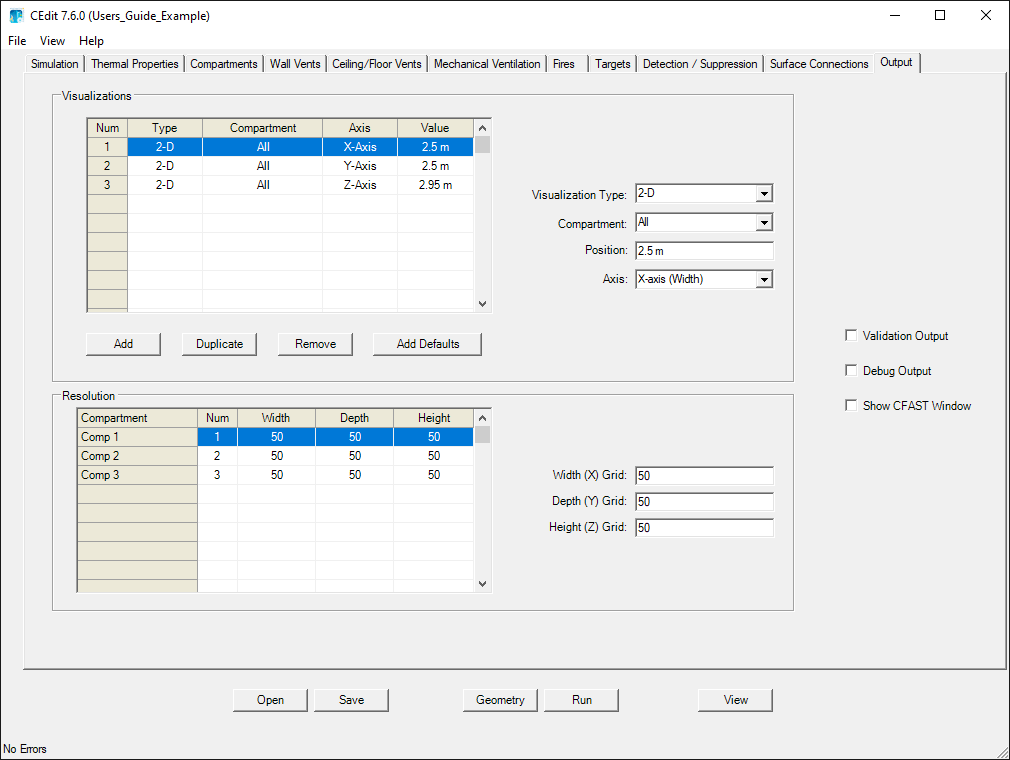
\includegraphics[width=6.5in]{FIGURES/Visualizations_Tab}
\caption[The CFAST Visualizations Tab]{The CFAST Visualizations Tab.}
\end{center}
\end{figure}

\section{Adding Visualizations}
\label{info:ISOF}
\label{info:SLCF}

\begin{description}
\item[Visualization Type] ( default value: 2-D): The type of visualization to be included. Choose from 2-D (a single plane slice of temperature at the position and axis specified), 3-D (a set of three animated slices whose position can be moved along its respective axis, or Isosurface (a fixed 3-D surface where the gas temperature is equal to the value specified. See the Smokeview documentation \cite{Smokeview_Users_Guide_6} for details on the use of Smokeview.

\item[Compartment] (default value: All): Visualizations can be placed in a single compartment or at the same position and axis in all compartments.

\item[Value] (default units: m, default value: 0 m): Position along the specified axes where the slice is placed measured from the compartment origin for the selected axis (0,0,0 is the bottom left corner of the compartment. See page \pageref{Compartment_Geometry}).

\item[Axis] (default value: X-axis (Width)): Axis perpendicular to the specified slice.  The slice is place perpendicular to the selected axis (the Y-Z plane for the X-Axis; the X-Z plane for the Y-Axis, and the X-Y plane for the Z-Axis)

\item[Temperature] (default units \degc, default value: none): Specified gas temperature for the selected isosurface.
\end{description}

%Not sure what is trying to be said here but I think it is a fail.
\graybox{
Use the Add Defaults button to add a default set of visualizations for the current simulation. A slice file entry is created at the center of each compartment in the x (width) and y (depth) directions along with one near the ceiling in the z direction. A 3-D slice file entry is created for each compartment as well.
}

\section{Visualization Resolution}
\label{info:SLCF2}

By default, slice files are generated with a grid of 50 data points in each direction for each compartment specified. If desired, the grid spacing can be adjusted up or down individually by compartment. Specifying a larger number of data points can \textit{dramatically} slow program execution since the gas temperature and velocity are evaluated at each grid location every time a Smokeview output is specified.  The default value should be appropriate for most simulations.

\begin{description}
\item[Width (X) Grid] (default unites: n/a, default value: 50): slices included along the X axis for each compartment are uniformly divided into the specified number of data points.

\item[Width (Y) Grid] (default unites: n/a, default value: 50): slices included along the Y axis for each compartment are uniformly divided into the specified number of data points.

\item[Width (Z) Grid] (default unites: n/a, default value: 50): slices included along the Z axis for each compartment are divided into the specified number of data points.
\end{description}

Sample visualizations are included below.

\begin{figure}[h!]
\begin{center}
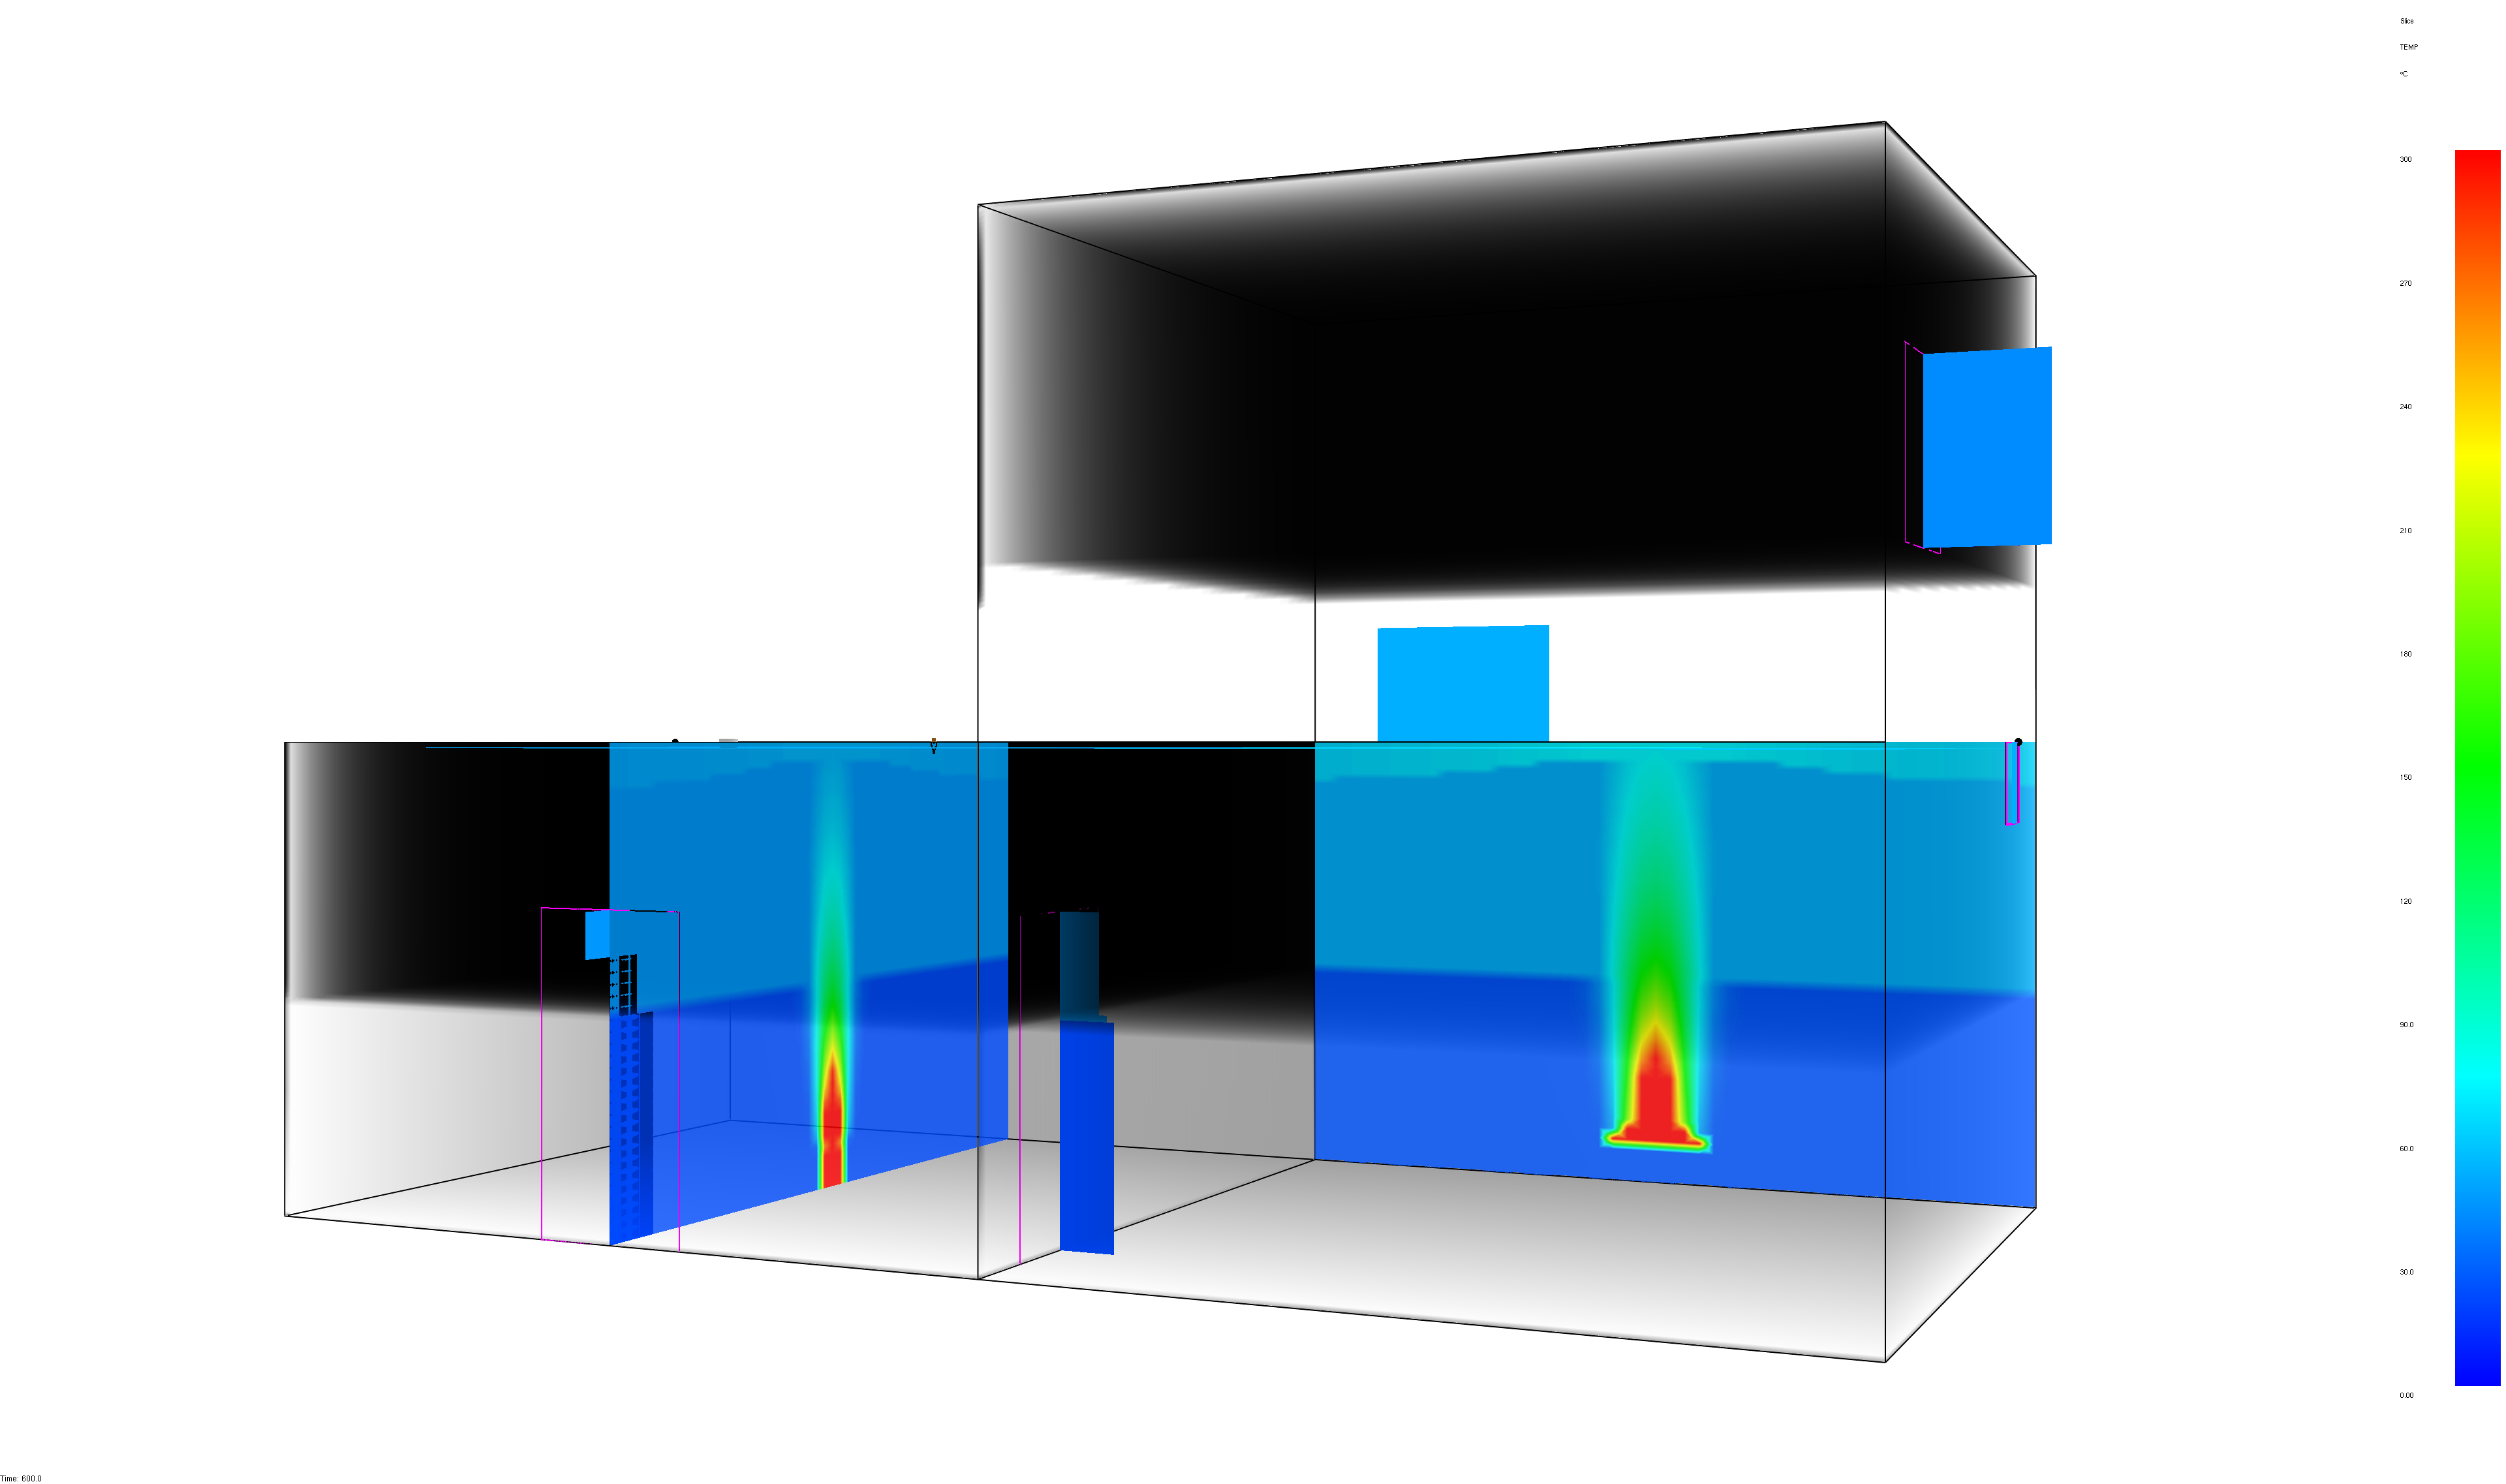
\includegraphics[width=6.5in]{FIGURES/SMV_Sample}
\caption{example Smokeview Visualization for a Three Compartment Test Case with Two Fires (\ct User\_Guide\_Example.in)}
\end{center}
\end{figure}

\begin{figure}[h!]
\begin{center}
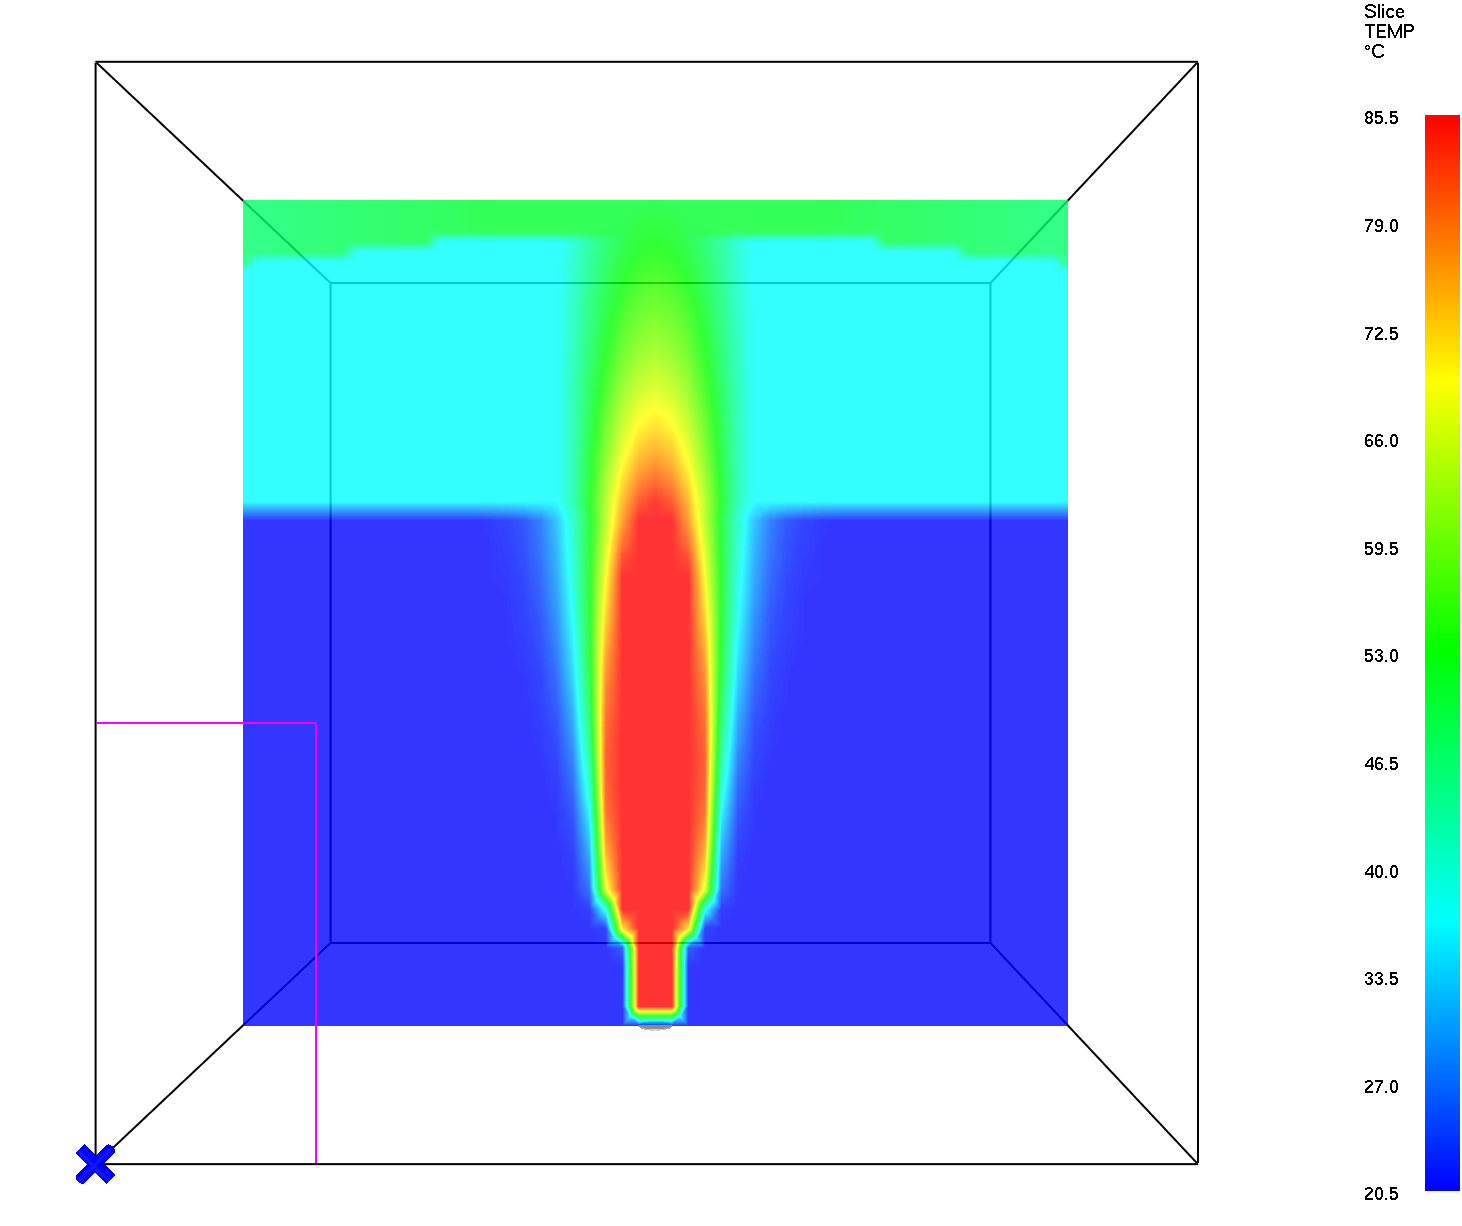
\includegraphics[width=6.5in]{FIGURES/SMV_Temperature}
\caption{Smokeview Visualization of Gas Temperature with a Single Fire}
\end{center}
\end{figure}

\begin{figure}[h!]
\begin{center}
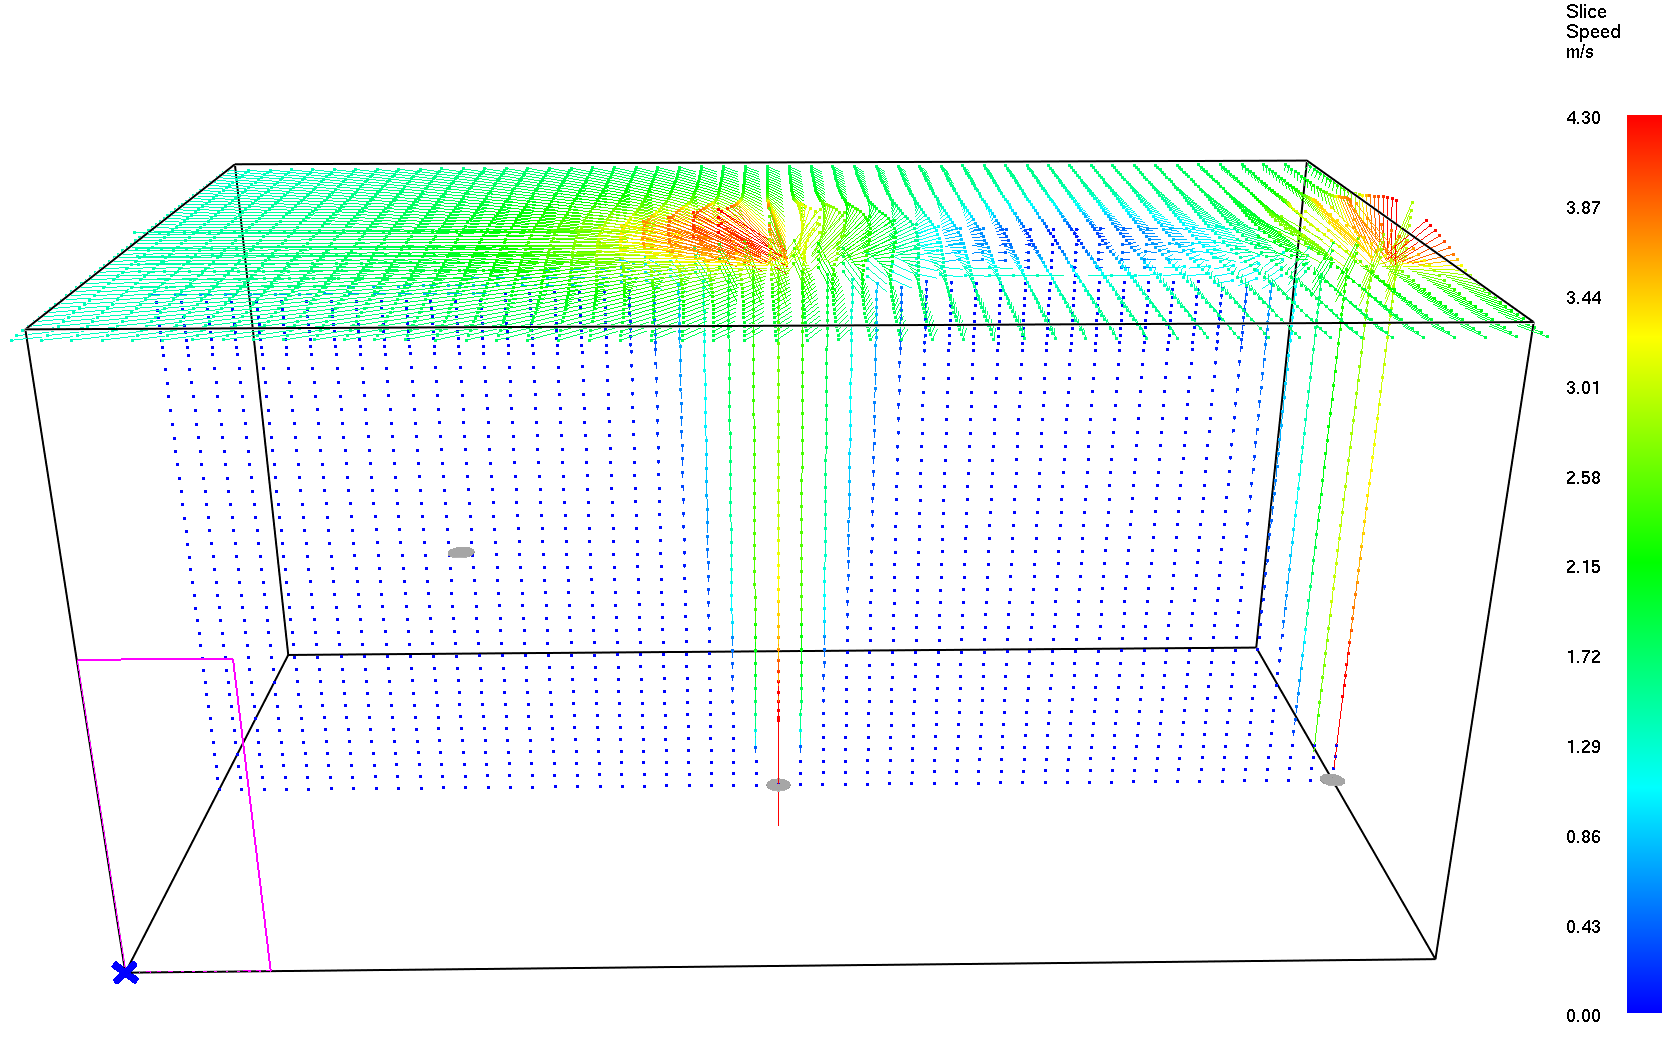
\includegraphics[width=6.5in]{FIGURES/SMV_Velocity}
\caption{Smokeview Visualization of Gas Velocity with Two Fires}
\end{center}
\end{figure}

\begin{figure}[h!]
\begin{center}
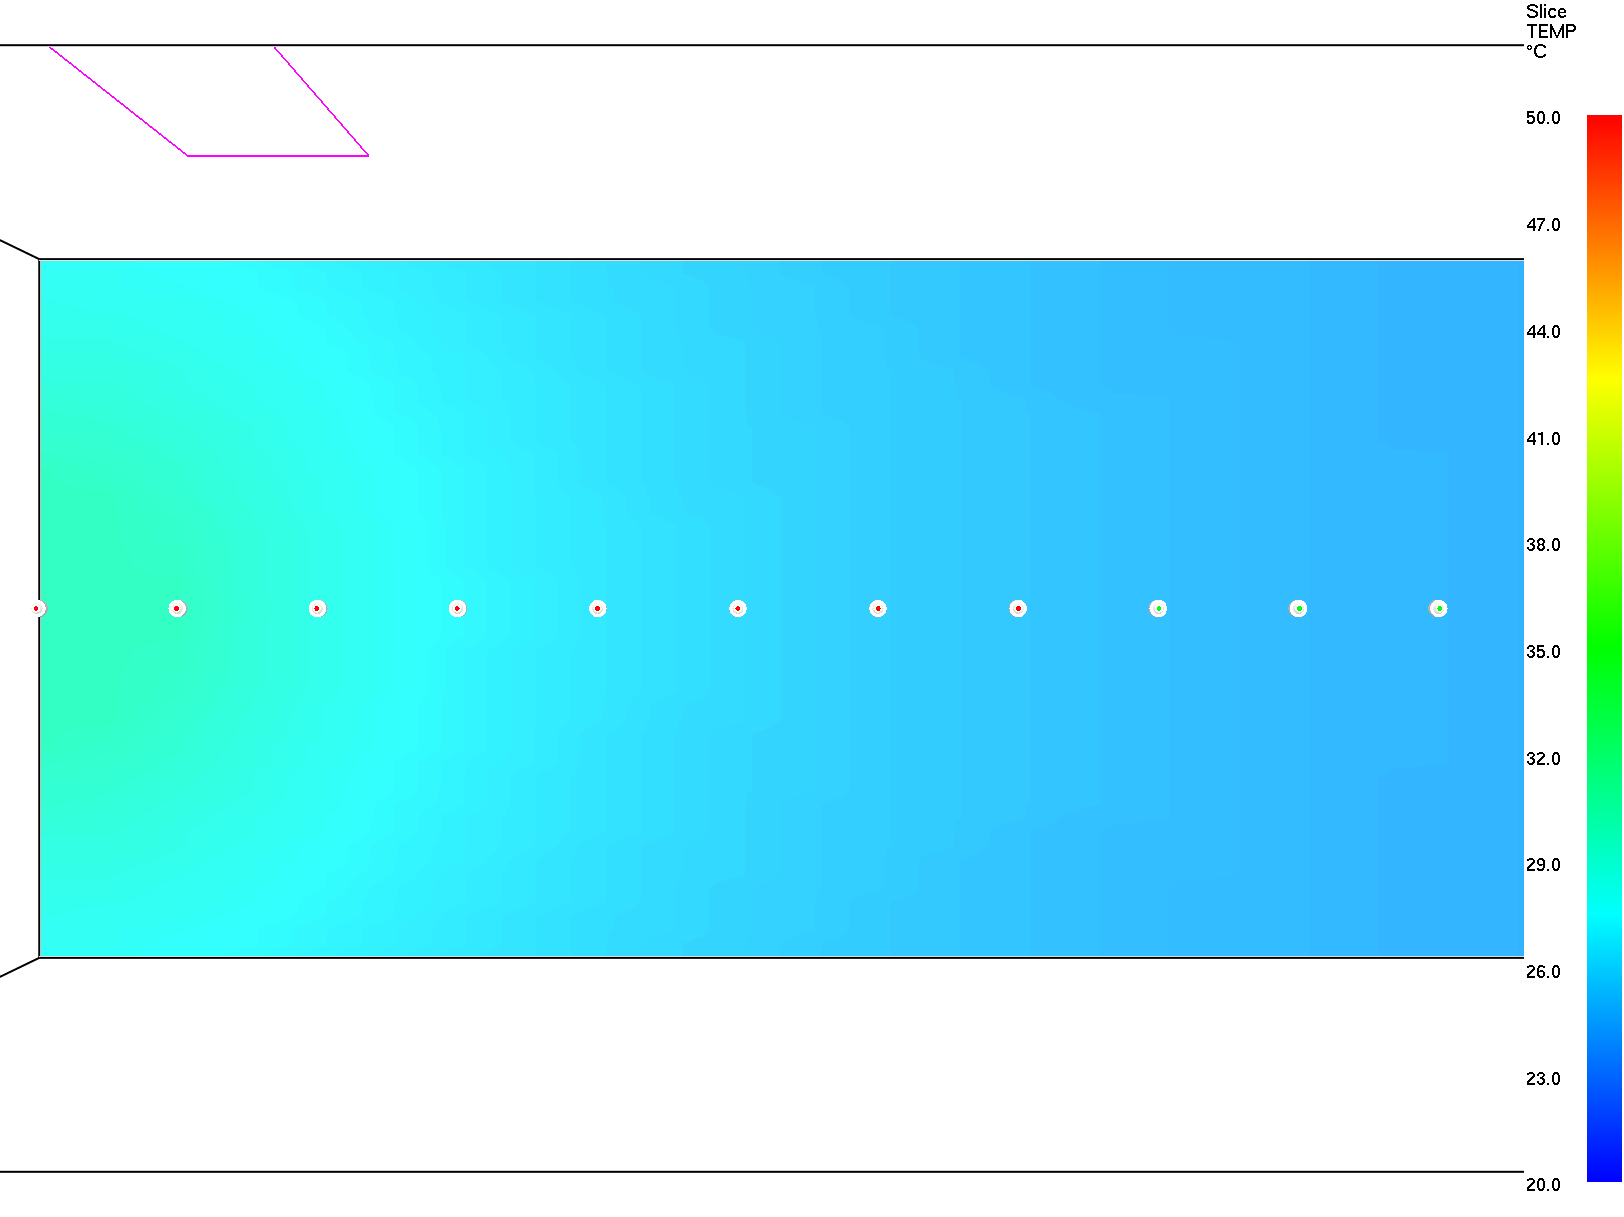
\includegraphics[width=6.5in]{FIGURES/SMV_Detectors}
\caption{Smokeview Visualization of Detector Activation in a Corridor}
\end{center}
\end{figure}

\section{Output Options}

By default, CFAST generates a set of output files that includes a formatted readable output and a set of spreadsheet files.  Options are available to modify the output files.  The default output should be appropriate for most simulations.

\begin{description}
    \item[CFAST Validation Output] If checked, this item directs the CFAST model to output abbreviated headings for spreadsheet columns that are better for automated processing of the data.
    \item[Debug Output] If checked, CFAST will create a detailed output spreadsheet that contains values of all the solution variables at each successful solution time step. This file is typically only of use to model developers diagnosing a problem with the model.
    \item[Show CFAST Window] If checked, this item allows the user to see the windows command prompt that is used to execute the CFAST model when the Model Simulation, CFAST menu item is used.  By default, this is not checked.  Normally, this can be left unchecked.  For troubleshooting, this can be selected to see additional details of the calculation as it progresses.
\end{description}




